\documentclass[twoside]{book}

% Packages required by doxygen
\usepackage{calc}
\usepackage{doxygen}
\usepackage{graphicx}
\usepackage[utf8]{inputenc}
\usepackage{makeidx}
\usepackage{multicol}
\usepackage{multirow}
\usepackage{textcomp}
\usepackage[table]{xcolor}

% Font selection
\usepackage[T1]{fontenc}
\usepackage{mathptmx}
\usepackage[scaled=.90]{helvet}
\usepackage{courier}
\usepackage{amssymb}
\usepackage{sectsty}
\renewcommand{\familydefault}{\sfdefault}
\allsectionsfont{%
  \fontseries{bc}\selectfont%
  \color{darkgray}%
}
\renewcommand{\DoxyLabelFont}{%
  \fontseries{bc}\selectfont%
  \color{darkgray}%
}

% Page & text layout
\usepackage{geometry}
\geometry{%
  letterpaper,%
  top=2.5cm,%
  bottom=2.5cm,%
  left=2.5cm,%
  right=2.5cm%
}
\tolerance=750
\hfuzz=15pt
\hbadness=750
\setlength{\emergencystretch}{15pt}
\setlength{\parindent}{0cm}
\setlength{\parskip}{0.2cm}
\makeatletter
\renewcommand{\paragraph}{%
  \@startsection{paragraph}{4}{0ex}{-1.0ex}{1.0ex}{%
    \normalfont\normalsize\bfseries\SS@parafont%
  }%
}
\renewcommand{\subparagraph}{%
  \@startsection{subparagraph}{5}{0ex}{-1.0ex}{1.0ex}{%
    \normalfont\normalsize\bfseries\SS@subparafont%
  }%
}
\makeatother

% Headers & footers
\usepackage{fancyhdr}
\pagestyle{fancyplain}
\fancyhead[LE]{\fancyplain{}{\bfseries\thepage}}
\fancyhead[CE]{\fancyplain{}{}}
\fancyhead[RE]{\fancyplain{}{\bfseries\leftmark}}
\fancyhead[LO]{\fancyplain{}{\bfseries\rightmark}}
\fancyhead[CO]{\fancyplain{}{}}
\fancyhead[RO]{\fancyplain{}{\bfseries\thepage}}
\fancyfoot[LE]{\fancyplain{}{}}
\fancyfoot[CE]{\fancyplain{}{}}
\fancyfoot[RE]{\fancyplain{}{\bfseries\scriptsize Generated on Mon Apr 27 2015 16\-:36\-:02 for 1-\/\-D S-\/2 Eulerian Radiation Hydrodynamics by Doxygen }}
\fancyfoot[LO]{\fancyplain{}{\bfseries\scriptsize Generated on Mon Apr 27 2015 16\-:36\-:02 for 1-\/\-D S-\/2 Eulerian Radiation Hydrodynamics by Doxygen }}
\fancyfoot[CO]{\fancyplain{}{}}
\fancyfoot[RO]{\fancyplain{}{}}
\renewcommand{\footrulewidth}{0.4pt}
\renewcommand{\chaptermark}[1]{%
  \markboth{#1}{}%
}
\renewcommand{\sectionmark}[1]{%
  \markright{\thesection\ #1}%
}

% Indices & bibliography
\usepackage{natbib}
\usepackage[titles]{tocloft}
\setcounter{tocdepth}{3}
\setcounter{secnumdepth}{5}
\makeindex

% Hyperlinks (required, but should be loaded last)
\usepackage{ifpdf}
\ifpdf
  \usepackage[pdftex,pagebackref=true]{hyperref}
\else
  \usepackage[ps2pdf,pagebackref=true]{hyperref}
\fi
\hypersetup{%
  colorlinks=true,%
  linkcolor=blue,%
  citecolor=blue,%
  unicode%
}

% Custom commands
\newcommand{\clearemptydoublepage}{%
  \newpage{\pagestyle{empty}\cleardoublepage}%
}


%===== C O N T E N T S =====

\begin{document}

% Titlepage & ToC
\hypersetup{pageanchor=false}
\pagenumbering{roman}
\begin{titlepage}
\vspace*{7cm}
\begin{center}%
{\Large 1-\/\-D S-\/2 Eulerian Radiation Hydrodynamics }\\
\vspace*{1cm}
{\large Generated by Doxygen 1.8.6}\\
\vspace*{0.5cm}
{\small Mon Apr 27 2015 16:36:02}\\
\end{center}
\end{titlepage}
\clearemptydoublepage
\tableofcontents
\clearemptydoublepage
\pagenumbering{arabic}
\hypersetup{pageanchor=true}

%--- Begin generated contents ---
\chapter{Namespace Index}
\section{Packages}
Here are the packages with brief descriptions (if available)\-:\begin{DoxyCompactList}
\item\contentsline{section}{\hyperlink{namespacesrc}{src} }{\pageref{namespacesrc}}{}
\item\contentsline{section}{\hyperlink{namespacesrc_1_1_cross_x_interface}{src.\-Cross\-X\-Interface} }{\pageref{namespacesrc_1_1_cross_x_interface}}{}
\item\contentsline{section}{\hyperlink{namespacesrc_1_1executioner}{src.\-executioner} }{\pageref{namespacesrc_1_1executioner}}{}
\item\contentsline{section}{\hyperlink{namespacesrc_1_1_mesh}{src.\-Mesh} }{\pageref{namespacesrc_1_1_mesh}}{}
\item\contentsline{section}{\hyperlink{namespacesrc_1_1_muscl_hanc}{src.\-Muscl\-Hanc} }{\pageref{namespacesrc_1_1_muscl_hanc}}{}
\item\contentsline{section}{\hyperlink{namespacesrc_1_1radiation_solver}{src.\-radiation\-Solver} }{\pageref{namespacesrc_1_1radiation_solver}}{}
\item\contentsline{section}{\hyperlink{namespacesrc_1_1utility_functions}{src.\-utility\-Functions} }{\pageref{namespacesrc_1_1utility_functions}}{}
\item\contentsline{section}{\hyperlink{namespace_this}{This} \\*Module contains helper functions }{\pageref{namespace_this}}{}
\end{DoxyCompactList}

\chapter{Hierarchical Index}
\section{Class Hierarchy}
This inheritance list is sorted roughly, but not completely, alphabetically\-:\begin{DoxyCompactList}
\item \contentsline{section}{Element}{\pageref{classsrc_1_1_mesh_1_1_element}}{}
\item \contentsline{section}{Hydro\-State}{\pageref{classsrc_1_1_muscl_hanc_1_1_hydro_state}}{}
\item \contentsline{section}{Mesh}{\pageref{classsrc_1_1_mesh_1_1_mesh}}{}
\item object\begin{DoxyCompactList}
\item \contentsline{section}{Cross\-X\-Interface}{\pageref{classsrc_1_1_cross_x_interface_1_1_cross_x_interface}}{}
\begin{DoxyCompactList}
\item \contentsline{section}{Inv\-Cubed\-Cross\-X}{\pageref{classsrc_1_1_cross_x_interface_1_1_inv_cubed_cross_x}}{}
\end{DoxyCompactList}
\end{DoxyCompactList}
\end{DoxyCompactList}

\chapter{Class Index}
\section{Class List}
Here are the classes, structs, unions and interfaces with brief descriptions\-:\begin{DoxyCompactList}
\item\contentsline{section}{\hyperlink{classsrc_1_1_cross_x_interface_1_1_cross_x_interface}{Cross\-X\-Interface} \\*Cross section class }{\pageref{classsrc_1_1_cross_x_interface_1_1_cross_x_interface}}{}
\item\contentsline{section}{\hyperlink{classsrc_1_1_mesh_1_1_element}{Element} }{\pageref{classsrc_1_1_mesh_1_1_element}}{}
\item\contentsline{section}{\hyperlink{classsrc_1_1_muscl_hanc_1_1_hydro_state}{Hydro\-State} }{\pageref{classsrc_1_1_muscl_hanc_1_1_hydro_state}}{}
\item\contentsline{section}{\hyperlink{classsrc_1_1_cross_x_interface_1_1_inv_cubed_cross_x}{Inv\-Cubed\-Cross\-X} \\*Inverse cubed cross section class }{\pageref{classsrc_1_1_cross_x_interface_1_1_inv_cubed_cross_x}}{}
\item\contentsline{section}{\hyperlink{classsrc_1_1_mesh_1_1_mesh}{Mesh} \\*Class for mesh }{\pageref{classsrc_1_1_mesh_1_1_mesh}}{}
\end{DoxyCompactList}

\chapter{File Index}
\section{File List}
Here is a list of all files with brief descriptions\-:\begin{DoxyCompactList}
\item\contentsline{section}{src/\hyperlink{____init_____8py}{\-\_\-\-\_\-init\-\_\-\-\_\-.\-py} }{\pageref{____init_____8py}}{}
\item\contentsline{section}{src/\hyperlink{_cross_x_interface_8py}{Cross\-X\-Interface.\-py} }{\pageref{_cross_x_interface_8py}}{}
\item\contentsline{section}{src/\hyperlink{executioner_8py}{executioner.\-py} }{\pageref{executioner_8py}}{}
\item\contentsline{section}{src/\hyperlink{_mesh_8py}{Mesh.\-py} }{\pageref{_mesh_8py}}{}
\item\contentsline{section}{src/\hyperlink{_muscl_hanc_8py}{Muscl\-Hanc.\-py} }{\pageref{_muscl_hanc_8py}}{}
\item\contentsline{section}{src/\hyperlink{radiation_solver_8py}{radiation\-Solver.\-py} }{\pageref{radiation_solver_8py}}{}
\item\contentsline{section}{src/\hyperlink{utility_functions_8py}{utility\-Functions.\-py} }{\pageref{utility_functions_8py}}{}
\end{DoxyCompactList}

\chapter{Namespace Documentation}
\hypertarget{namespacesrc}{\section{src Namespace Reference}
\label{namespacesrc}\index{src@{src}}
}
\subsection*{Namespaces}
\begin{DoxyCompactItemize}
\item 
\hyperlink{namespacesrc_1_1_cross_x_interface}{Cross\-X\-Interface}
\item 
\hyperlink{namespacesrc_1_1executioner}{executioner}
\item 
\hyperlink{namespacesrc_1_1_mesh}{Mesh}
\item 
\hyperlink{namespacesrc_1_1_muscl_hanc}{Muscl\-Hanc}
\item 
\hyperlink{namespacesrc_1_1radiation_solver}{radiation\-Solver}
\item 
\hyperlink{namespacesrc_1_1utility_functions}{utility\-Functions}
\end{DoxyCompactItemize}

\hypertarget{namespacesrc_1_1_cross_x_interface}{\section{src.\-Cross\-X\-Interface Namespace Reference}
\label{namespacesrc_1_1_cross_x_interface}\index{src.\-Cross\-X\-Interface@{src.\-Cross\-X\-Interface}}
}
\subsection*{Classes}
\begin{DoxyCompactItemize}
\item 
class \hyperlink{classsrc_1_1_cross_x_interface_1_1_cross_x_interface}{Cross\-X\-Interface}
\begin{DoxyCompactList}\small\item\em Cross section class. \end{DoxyCompactList}\item 
class \hyperlink{classsrc_1_1_cross_x_interface_1_1_inv_cubed_cross_x}{Inv\-Cubed\-Cross\-X}
\begin{DoxyCompactList}\small\item\em Inverse cubed cross section class. \end{DoxyCompactList}\end{DoxyCompactItemize}

\hypertarget{namespacesrc_1_1executioner}{\section{src.\-executioner Namespace Reference}
\label{namespacesrc_1_1executioner}\index{src.\-executioner@{src.\-executioner}}
}
\subsection*{Functions}
\begin{DoxyCompactItemize}
\item 
def \hyperlink{namespacesrc_1_1executioner_a95244228b76d454293329ede466072c2}{solve\-Hydro\-Problem}
\begin{DoxyCompactList}\small\item\em Main executioner for Hydro solve. \end{DoxyCompactList}\end{DoxyCompactItemize}


\subsection{Function Documentation}
\hypertarget{namespacesrc_1_1executioner_a95244228b76d454293329ede466072c2}{\index{src\-::executioner@{src\-::executioner}!solve\-Hydro\-Problem@{solve\-Hydro\-Problem}}
\index{solve\-Hydro\-Problem@{solve\-Hydro\-Problem}!src::executioner@{src\-::executioner}}
\subsubsection[{solve\-Hydro\-Problem}]{\setlength{\rightskip}{0pt plus 5cm}def src.\-executioner.\-solve\-Hydro\-Problem (
\begin{DoxyParamCaption}
{}
\end{DoxyParamCaption}
)}}\label{namespacesrc_1_1executioner_a95244228b76d454293329ede466072c2}


Main executioner for Hydro solve. 

Currently in a testing state.


\begin{DoxyParams}[1]{Parameters}
\mbox{\tt in}  & {\em mesh} & a mesh object \\
\hline
\mbox{\tt in}  & {\em cross\-\_\-x} & list of cross sections for each element \\
\hline
\mbox{\tt in}  & {\em Q0} & isotropic source \\
\hline
\mbox{\tt in}  & {\em Q1\-\_\-plus} & source for plus directions \\
\hline
\mbox{\tt in}  & {\em Q1\-\_\-minus} & source for minus directions \\
\hline
\mbox{\tt in}  & {\em stream\-\_\-scale\-\_\-factor} & scale factor for reaction and streaming terms \\
\hline
\mbox{\tt in}  & {\em diag\-\_\-add\-\_\-term} & term to add to reaction term \\
\hline
\mbox{\tt in}  & {\em bound\-\_\-curr\-\_\-lt} & left boundary current \\
\hline
\mbox{\tt in}  & {\em bound\-\_\-curr\-\_\-rt} & right boundary current\\
\hline
\end{DoxyParams}
\begin{DoxyReturn}{Returns}

\begin{DoxyEnumerate}
\item $\psi^+$, angular flux in plus directions
\item $\psi^-$, angular flux in minus directions
\item $\mathcal{E}$\-: radiation energy
\item $\mathcal{F}$\-: radiation flux 
\end{DoxyEnumerate}
\end{DoxyReturn}

\hypertarget{namespacesrc_1_1_mesh}{\section{src.\-Mesh Namespace Reference}
\label{namespacesrc_1_1_mesh}\index{src.\-Mesh@{src.\-Mesh}}
}
\subsection*{Classes}
\begin{DoxyCompactItemize}
\item 
class \hyperlink{classsrc_1_1_mesh_1_1_element}{Element}
\item 
class \hyperlink{classsrc_1_1_mesh_1_1_mesh}{Mesh}
\begin{DoxyCompactList}\small\item\em Class for mesh. \end{DoxyCompactList}\end{DoxyCompactItemize}

\hypertarget{namespacesrc_1_1_muscl_hanc}{\section{src.\-Muscl\-Hanc Namespace Reference}
\label{namespacesrc_1_1_muscl_hanc}\index{src.\-Muscl\-Hanc@{src.\-Muscl\-Hanc}}
}
\subsection*{Classes}
\begin{DoxyCompactItemize}
\item 
class \hyperlink{classsrc_1_1_muscl_hanc_1_1_hydro_state}{Hydro\-State}
\end{DoxyCompactItemize}
\subsection*{Functions}
\begin{DoxyCompactItemize}
\item 
def \hyperlink{namespacesrc_1_1_muscl_hanc_ade24903eca1238058267cd23d9d801fc}{adv\-Cons}
\item 
def \hyperlink{namespacesrc_1_1_muscl_hanc_ad23caa5b14e969c440cf2b252fd6b1a2}{erg\-Flux}
\item 
def \hyperlink{namespacesrc_1_1_muscl_hanc_afe1723988c5a5267d18ff9476df89790}{get\-Int\-Erg}
\item 
def \hyperlink{namespacesrc_1_1_muscl_hanc_a2d178cf1cadff5d732656c30f2a9b861}{get\-Pressure}
\item 
def \hyperlink{namespacesrc_1_1_muscl_hanc_ae2ddd173a646e89b12c2461f5c45874a}{get\-Volume}
\item 
def \hyperlink{namespacesrc_1_1_muscl_hanc_a03a9255024224353a0170b402f09fa80}{H\-L\-L\-C\-Solver}
\item 
def \hyperlink{namespacesrc_1_1_muscl_hanc_a38faa5e281253b4325d831e07ad88666}{H\-L\-L\-Solver}
\item 
def \hyperlink{namespacesrc_1_1_muscl_hanc_ab9ce990167303930a361b03f3c230726}{hydro\-Corrector}
\begin{DoxyCompactList}\small\item\em Corrector solver for hydro. \end{DoxyCompactList}\item 
def \hyperlink{namespacesrc_1_1_muscl_hanc_a5a28a779b62a90fc19782d2814eb4dc9}{hydro\-Predictor}
\begin{DoxyCompactList}\small\item\em Predictor solver for hydro. \end{DoxyCompactList}\item 
def \hyperlink{namespacesrc_1_1_muscl_hanc_a580462093ccf4bf9a916537de4935caf}{main}
\begin{DoxyCompactList}\small\item\em Main is my original hydro code, we shouldnt need this anymore. \end{DoxyCompactList}\item 
def \hyperlink{namespacesrc_1_1_muscl_hanc_a39159a54fe21dc897f761cefa0f6314a}{min\-Mod}
\item 
def \hyperlink{namespacesrc_1_1_muscl_hanc_a009e09e7699202cbefd6ded237fc58d6}{mom\-Flux}
\item 
def \hyperlink{namespacesrc_1_1_muscl_hanc_a7f1a3ce6fe8741016cb4eadd253391ae}{plot2\-D}
\item 
def \hyperlink{namespacesrc_1_1_muscl_hanc_aeee7e33a3d044d1ae221fbfb9cf0e9f2}{plot\-Hydro\-Solutions}
\item 
def \hyperlink{namespacesrc_1_1_muscl_hanc_a1a1f834022191e3ac8aed54a6aad3890}{plot\-Single}
\item 
def \hyperlink{namespacesrc_1_1_muscl_hanc_adfc329f2e09f5773b1296111868d1ddb}{rho\-Flux}
\item 
def \hyperlink{namespacesrc_1_1_muscl_hanc_aa761b91519d89b31df5507bffd2ef7de}{slope\-Reconstruction}
\end{DoxyCompactItemize}


\subsection{Function Documentation}
\hypertarget{namespacesrc_1_1_muscl_hanc_ade24903eca1238058267cd23d9d801fc}{\index{src\-::\-Muscl\-Hanc@{src\-::\-Muscl\-Hanc}!adv\-Cons@{adv\-Cons}}
\index{adv\-Cons@{adv\-Cons}!src::MusclHanc@{src\-::\-Muscl\-Hanc}}
\subsubsection[{adv\-Cons}]{\setlength{\rightskip}{0pt plus 5cm}def src.\-Muscl\-Hanc.\-adv\-Cons (
\begin{DoxyParamCaption}
\item[{}]{val, }
\item[{}]{dx, }
\item[{}]{dt, }
\item[{}]{f\-\_\-left, }
\item[{}]{f\-\_\-right}
\end{DoxyParamCaption}
)}}\label{namespacesrc_1_1_muscl_hanc_ade24903eca1238058267cd23d9d801fc}
\hypertarget{namespacesrc_1_1_muscl_hanc_ad23caa5b14e969c440cf2b252fd6b1a2}{\index{src\-::\-Muscl\-Hanc@{src\-::\-Muscl\-Hanc}!erg\-Flux@{erg\-Flux}}
\index{erg\-Flux@{erg\-Flux}!src::MusclHanc@{src\-::\-Muscl\-Hanc}}
\subsubsection[{erg\-Flux}]{\setlength{\rightskip}{0pt plus 5cm}def src.\-Muscl\-Hanc.\-erg\-Flux (
\begin{DoxyParamCaption}
\item[{}]{s}
\end{DoxyParamCaption}
)}}\label{namespacesrc_1_1_muscl_hanc_ad23caa5b14e969c440cf2b252fd6b1a2}
\hypertarget{namespacesrc_1_1_muscl_hanc_afe1723988c5a5267d18ff9476df89790}{\index{src\-::\-Muscl\-Hanc@{src\-::\-Muscl\-Hanc}!get\-Int\-Erg@{get\-Int\-Erg}}
\index{get\-Int\-Erg@{get\-Int\-Erg}!src::MusclHanc@{src\-::\-Muscl\-Hanc}}
\subsubsection[{get\-Int\-Erg}]{\setlength{\rightskip}{0pt plus 5cm}def src.\-Muscl\-Hanc.\-get\-Int\-Erg (
\begin{DoxyParamCaption}
\item[{}]{gamma, }
\item[{}]{rho, }
\item[{}]{p}
\end{DoxyParamCaption}
)}}\label{namespacesrc_1_1_muscl_hanc_afe1723988c5a5267d18ff9476df89790}
\hypertarget{namespacesrc_1_1_muscl_hanc_a2d178cf1cadff5d732656c30f2a9b861}{\index{src\-::\-Muscl\-Hanc@{src\-::\-Muscl\-Hanc}!get\-Pressure@{get\-Pressure}}
\index{get\-Pressure@{get\-Pressure}!src::MusclHanc@{src\-::\-Muscl\-Hanc}}
\subsubsection[{get\-Pressure}]{\setlength{\rightskip}{0pt plus 5cm}def src.\-Muscl\-Hanc.\-get\-Pressure (
\begin{DoxyParamCaption}
\item[{}]{gamma, }
\item[{}]{rho, }
\item[{}]{e}
\end{DoxyParamCaption}
)}}\label{namespacesrc_1_1_muscl_hanc_a2d178cf1cadff5d732656c30f2a9b861}
\hypertarget{namespacesrc_1_1_muscl_hanc_ae2ddd173a646e89b12c2461f5c45874a}{\index{src\-::\-Muscl\-Hanc@{src\-::\-Muscl\-Hanc}!get\-Volume@{get\-Volume}}
\index{get\-Volume@{get\-Volume}!src::MusclHanc@{src\-::\-Muscl\-Hanc}}
\subsubsection[{get\-Volume}]{\setlength{\rightskip}{0pt plus 5cm}def src.\-Muscl\-Hanc.\-get\-Volume (
\begin{DoxyParamCaption}
\item[{}]{x1, }
\item[{}]{x2}
\end{DoxyParamCaption}
)}}\label{namespacesrc_1_1_muscl_hanc_ae2ddd173a646e89b12c2461f5c45874a}
\hypertarget{namespacesrc_1_1_muscl_hanc_a03a9255024224353a0170b402f09fa80}{\index{src\-::\-Muscl\-Hanc@{src\-::\-Muscl\-Hanc}!H\-L\-L\-C\-Solver@{H\-L\-L\-C\-Solver}}
\index{H\-L\-L\-C\-Solver@{H\-L\-L\-C\-Solver}!src::MusclHanc@{src\-::\-Muscl\-Hanc}}
\subsubsection[{H\-L\-L\-C\-Solver}]{\setlength{\rightskip}{0pt plus 5cm}def src.\-Muscl\-Hanc.\-H\-L\-L\-C\-Solver (
\begin{DoxyParamCaption}
\item[{}]{U\-\_\-l, }
\item[{}]{U\-\_\-r, }
\item[{}]{L, }
\item[{}]{R, }
\item[{}]{flux}
\end{DoxyParamCaption}
)}}\label{namespacesrc_1_1_muscl_hanc_a03a9255024224353a0170b402f09fa80}
\hypertarget{namespacesrc_1_1_muscl_hanc_a38faa5e281253b4325d831e07ad88666}{\index{src\-::\-Muscl\-Hanc@{src\-::\-Muscl\-Hanc}!H\-L\-L\-Solver@{H\-L\-L\-Solver}}
\index{H\-L\-L\-Solver@{H\-L\-L\-Solver}!src::MusclHanc@{src\-::\-Muscl\-Hanc}}
\subsubsection[{H\-L\-L\-Solver}]{\setlength{\rightskip}{0pt plus 5cm}def src.\-Muscl\-Hanc.\-H\-L\-L\-Solver (
\begin{DoxyParamCaption}
\item[{}]{U\-\_\-l, }
\item[{}]{U\-\_\-r, }
\item[{}]{L, }
\item[{}]{R, }
\item[{}]{flux}
\end{DoxyParamCaption}
)}}\label{namespacesrc_1_1_muscl_hanc_a38faa5e281253b4325d831e07ad88666}
\hypertarget{namespacesrc_1_1_muscl_hanc_ab9ce990167303930a361b03f3c230726}{\index{src\-::\-Muscl\-Hanc@{src\-::\-Muscl\-Hanc}!hydro\-Corrector@{hydro\-Corrector}}
\index{hydro\-Corrector@{hydro\-Corrector}!src::MusclHanc@{src\-::\-Muscl\-Hanc}}
\subsubsection[{hydro\-Corrector}]{\setlength{\rightskip}{0pt plus 5cm}def src.\-Muscl\-Hanc.\-hydro\-Corrector (
\begin{DoxyParamCaption}
\item[{}]{mesh, }
\item[{}]{states\-\_\-old\-\_\-a, }
\item[{}]{states\-\_\-l, }
\item[{}]{states\-\_\-r, }
\item[{}]{dt}
\end{DoxyParamCaption}
)}}\label{namespacesrc_1_1_muscl_hanc_ab9ce990167303930a361b03f3c230726}


Corrector solver for hydro. 

The corrector solve takes in a predicted state at dt/2, and computes new values at dt. The input is averages and slopes, the output is new averages, with the slopes un-\/adjusted.

The slopes are defined based on the following relation in a cell\-:

$U(x) = U_a + \frac{2U_x}{h_x}(x - x_i) $

Thus, $U_R = U_a + U_x$ and $U_L = U_a - U_x$, and $U_x = \frac{U_R - U_L}{2}$


\begin{DoxyParams}[1]{Parameters}
\mbox{\tt in}  & {\em mesh} & Basic spatial mesh object \\
\hline
\mbox{\tt in}  & {\em states\-\_\-old\-\_\-a} & Averages at old state. \\
\hline
\mbox{\tt in}  & {\em states\-\_\-l} & Predicted values at left nodes, at dt/2 \\
\hline
\mbox{\tt in}  & {\em states\-\_\-r} & Predicted values at right nodes, at dt/2 \\
\hline
\mbox{\tt in}  & {\em delta\-\_\-t} & time step size for this hydro solve. To predict values at 0.\-5 dt, pass in 1.\-0 dt\\
\hline
\end{DoxyParams}
\begin{DoxyReturn}{Returns}

\begin{DoxyEnumerate}
\item predicted states averages 
\end{DoxyEnumerate}
\end{DoxyReturn}
\hypertarget{namespacesrc_1_1_muscl_hanc_a5a28a779b62a90fc19782d2814eb4dc9}{\index{src\-::\-Muscl\-Hanc@{src\-::\-Muscl\-Hanc}!hydro\-Predictor@{hydro\-Predictor}}
\index{hydro\-Predictor@{hydro\-Predictor}!src::MusclHanc@{src\-::\-Muscl\-Hanc}}
\subsubsection[{hydro\-Predictor}]{\setlength{\rightskip}{0pt plus 5cm}def src.\-Muscl\-Hanc.\-hydro\-Predictor (
\begin{DoxyParamCaption}
\item[{}]{mesh, }
\item[{}]{states\-\_\-old\-\_\-a, }
\item[{}]{dt}
\end{DoxyParamCaption}
)}}\label{namespacesrc_1_1_muscl_hanc_a5a28a779b62a90fc19782d2814eb4dc9}


Predictor solver for hydro. 

Boundary Conditions\-: Essentially boundaries are treated as reflective. The fluxes on the boundary are just estimated based on the flux based on the edge state at that node. There is no need to pass in the boundary conditions then.


\begin{DoxyParams}[1]{Parameters}
\mbox{\tt in}  & {\em mesh} & Basic spatial mesh object \\
\hline
\mbox{\tt in}  & {\em states\-\_\-old\-\_\-a} & Averages at old state. \\
\hline
\mbox{\tt in}  & {\em dt} & time step size for this hydro solve. To predict values at 0.\-5 dt, pass in 1.\-0 dt\\
\hline
\end{DoxyParams}
\begin{DoxyReturn}{Returns}

\begin{DoxyEnumerate}
\item predicted states at averages
\item predicted states slopes 
\end{DoxyEnumerate}
\end{DoxyReturn}
\hypertarget{namespacesrc_1_1_muscl_hanc_a580462093ccf4bf9a916537de4935caf}{\index{src\-::\-Muscl\-Hanc@{src\-::\-Muscl\-Hanc}!main@{main}}
\index{main@{main}!src::MusclHanc@{src\-::\-Muscl\-Hanc}}
\subsubsection[{main}]{\setlength{\rightskip}{0pt plus 5cm}def src.\-Muscl\-Hanc.\-main (
\begin{DoxyParamCaption}
{}
\end{DoxyParamCaption}
)}}\label{namespacesrc_1_1_muscl_hanc_a580462093ccf4bf9a916537de4935caf}


Main is my original hydro code, we shouldnt need this anymore. 

\hypertarget{namespacesrc_1_1_muscl_hanc_a39159a54fe21dc897f761cefa0f6314a}{\index{src\-::\-Muscl\-Hanc@{src\-::\-Muscl\-Hanc}!min\-Mod@{min\-Mod}}
\index{min\-Mod@{min\-Mod}!src::MusclHanc@{src\-::\-Muscl\-Hanc}}
\subsubsection[{min\-Mod}]{\setlength{\rightskip}{0pt plus 5cm}def src.\-Muscl\-Hanc.\-min\-Mod (
\begin{DoxyParamCaption}
\item[{}]{a, }
\item[{}]{b}
\end{DoxyParamCaption}
)}}\label{namespacesrc_1_1_muscl_hanc_a39159a54fe21dc897f761cefa0f6314a}
\hypertarget{namespacesrc_1_1_muscl_hanc_a009e09e7699202cbefd6ded237fc58d6}{\index{src\-::\-Muscl\-Hanc@{src\-::\-Muscl\-Hanc}!mom\-Flux@{mom\-Flux}}
\index{mom\-Flux@{mom\-Flux}!src::MusclHanc@{src\-::\-Muscl\-Hanc}}
\subsubsection[{mom\-Flux}]{\setlength{\rightskip}{0pt plus 5cm}def src.\-Muscl\-Hanc.\-mom\-Flux (
\begin{DoxyParamCaption}
\item[{}]{s}
\end{DoxyParamCaption}
)}}\label{namespacesrc_1_1_muscl_hanc_a009e09e7699202cbefd6ded237fc58d6}
\hypertarget{namespacesrc_1_1_muscl_hanc_a7f1a3ce6fe8741016cb4eadd253391ae}{\index{src\-::\-Muscl\-Hanc@{src\-::\-Muscl\-Hanc}!plot2\-D@{plot2\-D}}
\index{plot2\-D@{plot2\-D}!src::MusclHanc@{src\-::\-Muscl\-Hanc}}
\subsubsection[{plot2\-D}]{\setlength{\rightskip}{0pt plus 5cm}def src.\-Muscl\-Hanc.\-plot2\-D (
\begin{DoxyParamCaption}
\item[{}]{x, }
\item[{}]{y, }
\item[{}]{x\-\_\-ex, }
\item[{}]{y\-\_\-ex, }
\item[{}]{ylabl}
\end{DoxyParamCaption}
)}}\label{namespacesrc_1_1_muscl_hanc_a7f1a3ce6fe8741016cb4eadd253391ae}
\hypertarget{namespacesrc_1_1_muscl_hanc_aeee7e33a3d044d1ae221fbfb9cf0e9f2}{\index{src\-::\-Muscl\-Hanc@{src\-::\-Muscl\-Hanc}!plot\-Hydro\-Solutions@{plot\-Hydro\-Solutions}}
\index{plot\-Hydro\-Solutions@{plot\-Hydro\-Solutions}!src::MusclHanc@{src\-::\-Muscl\-Hanc}}
\subsubsection[{plot\-Hydro\-Solutions}]{\setlength{\rightskip}{0pt plus 5cm}def src.\-Muscl\-Hanc.\-plot\-Hydro\-Solutions (
\begin{DoxyParamCaption}
\item[{}]{x, }
\item[{}]{states = {\ttfamily None}}
\end{DoxyParamCaption}
)}}\label{namespacesrc_1_1_muscl_hanc_aeee7e33a3d044d1ae221fbfb9cf0e9f2}
\hypertarget{namespacesrc_1_1_muscl_hanc_a1a1f834022191e3ac8aed54a6aad3890}{\index{src\-::\-Muscl\-Hanc@{src\-::\-Muscl\-Hanc}!plot\-Single@{plot\-Single}}
\index{plot\-Single@{plot\-Single}!src::MusclHanc@{src\-::\-Muscl\-Hanc}}
\subsubsection[{plot\-Single}]{\setlength{\rightskip}{0pt plus 5cm}def src.\-Muscl\-Hanc.\-plot\-Single (
\begin{DoxyParamCaption}
\item[{}]{x, }
\item[{}]{y, }
\item[{}]{ylabl}
\end{DoxyParamCaption}
)}}\label{namespacesrc_1_1_muscl_hanc_a1a1f834022191e3ac8aed54a6aad3890}
\hypertarget{namespacesrc_1_1_muscl_hanc_adfc329f2e09f5773b1296111868d1ddb}{\index{src\-::\-Muscl\-Hanc@{src\-::\-Muscl\-Hanc}!rho\-Flux@{rho\-Flux}}
\index{rho\-Flux@{rho\-Flux}!src::MusclHanc@{src\-::\-Muscl\-Hanc}}
\subsubsection[{rho\-Flux}]{\setlength{\rightskip}{0pt plus 5cm}def src.\-Muscl\-Hanc.\-rho\-Flux (
\begin{DoxyParamCaption}
\item[{}]{s}
\end{DoxyParamCaption}
)}}\label{namespacesrc_1_1_muscl_hanc_adfc329f2e09f5773b1296111868d1ddb}
\hypertarget{namespacesrc_1_1_muscl_hanc_aa761b91519d89b31df5507bffd2ef7de}{\index{src\-::\-Muscl\-Hanc@{src\-::\-Muscl\-Hanc}!slope\-Reconstruction@{slope\-Reconstruction}}
\index{slope\-Reconstruction@{slope\-Reconstruction}!src::MusclHanc@{src\-::\-Muscl\-Hanc}}
\subsubsection[{slope\-Reconstruction}]{\setlength{\rightskip}{0pt plus 5cm}def src.\-Muscl\-Hanc.\-slope\-Reconstruction (
\begin{DoxyParamCaption}
\item[{}]{u}
\end{DoxyParamCaption}
)}}\label{namespacesrc_1_1_muscl_hanc_aa761b91519d89b31df5507bffd2ef7de}

\hypertarget{namespacesrc_1_1radiation_solver}{\section{src.\-radiation\-Solver Namespace Reference}
\label{namespacesrc_1_1radiation_solver}\index{src.\-radiation\-Solver@{src.\-radiation\-Solver}}
}
\subsection*{Functions}
\begin{DoxyCompactItemize}
\item 
def \hyperlink{namespacesrc_1_1radiation_solver_a7c6794c1be4b79d2c09154579ff6a06c}{radiation\-Solver}
\begin{DoxyCompactList}\small\item\em Steady-\/state solve function for the S-\/2 equations. \end{DoxyCompactList}\end{DoxyCompactItemize}


\subsection{Function Documentation}
\hypertarget{namespacesrc_1_1radiation_solver_a7c6794c1be4b79d2c09154579ff6a06c}{\index{src\-::radiation\-Solver@{src\-::radiation\-Solver}!radiation\-Solver@{radiation\-Solver}}
\index{radiation\-Solver@{radiation\-Solver}!src::radiationSolver@{src\-::radiation\-Solver}}
\subsubsection[{radiation\-Solver}]{\setlength{\rightskip}{0pt plus 5cm}def src.\-radiation\-Solver.\-radiation\-Solver (
\begin{DoxyParamCaption}
\item[{}]{mesh, }
\item[{}]{cross\-\_\-x, }
\item[{}]{Q0, }
\item[{}]{Q1\-\_\-plus, }
\item[{}]{Q1\-\_\-minus, }
\item[{}]{stream\-\_\-scale\-\_\-factor = {\ttfamily 1.0}, }
\item[{}]{diag\-\_\-add\-\_\-term = {\ttfamily 0.0}, }
\item[{}]{bound\-\_\-curr\-\_\-lt = {\ttfamily 0.0}, }
\item[{}]{bound\-\_\-curr\-\_\-rt = {\ttfamily 0.0}}
\end{DoxyParamCaption}
)}}\label{namespacesrc_1_1radiation_solver_a7c6794c1be4b79d2c09154579ff6a06c}


Steady-\/state solve function for the S-\/2 equations. 


\begin{DoxyParams}[1]{Parameters}
\mbox{\tt in}  & {\em mesh} & a mesh object \\
\hline
\mbox{\tt in}  & {\em cross\-\_\-x} & list of cross sections for each element \\
\hline
\mbox{\tt in}  & {\em Q0} & isotropic source \\
\hline
\mbox{\tt in}  & {\em Q1\-\_\-plus} & source for plus directions \\
\hline
\mbox{\tt in}  & {\em Q1\-\_\-minus} & source for minus directions \\
\hline
\mbox{\tt in}  & {\em stream\-\_\-scale\-\_\-factor} & scale factor for reaction and streaming terms \\
\hline
\mbox{\tt in}  & {\em diag\-\_\-add\-\_\-term} & term to add to reaction term \\
\hline
\mbox{\tt in}  & {\em bound\-\_\-curr\-\_\-lt} & left boundary current \\
\hline
\mbox{\tt in}  & {\em bound\-\_\-curr\-\_\-rt} & right boundary current\\
\hline
\end{DoxyParams}
\begin{DoxyReturn}{Returns}

\begin{DoxyEnumerate}
\item $\psi^+$, angular flux in plus directions
\item $\psi^-$, angular flux in minus directions
\item $\mathcal{E}$\-: radiation energy
\item $\mathcal{F}$\-: radiation flux 
\end{DoxyEnumerate}
\end{DoxyReturn}

\hypertarget{namespacesrc_1_1utility_functions}{\section{src.\-utility\-Functions Namespace Reference}
\label{namespacesrc_1_1utility_functions}\index{src.\-utility\-Functions@{src.\-utility\-Functions}}
}
\subsection*{Functions}
\begin{DoxyCompactItemize}
\item 
def \hyperlink{namespacesrc_1_1utility_functions_aaecb6735e6d21d8bcd4cbb4a6bd8e1b2}{Edg\-To\-Mom}
\begin{DoxyCompactList}\small\item\em Converge f\-\_\-\-L and f\-\_\-\-R to f\-\_\-a and f\-\_\-x. \end{DoxyCompactList}\item 
def \hyperlink{namespacesrc_1_1utility_functions_ae6b69f9a3bb74164b3526a2d9ca49c3d}{Mom\-To\-Edg}
\begin{DoxyCompactList}\small\item\em Converge f\-\_\-x and f\-\_\-a to f\-\_\-l and f\-\_\-r. \end{DoxyCompactList}\end{DoxyCompactItemize}


\subsection{Function Documentation}
\hypertarget{namespacesrc_1_1utility_functions_aaecb6735e6d21d8bcd4cbb4a6bd8e1b2}{\index{src\-::utility\-Functions@{src\-::utility\-Functions}!Edg\-To\-Mom@{Edg\-To\-Mom}}
\index{Edg\-To\-Mom@{Edg\-To\-Mom}!src::utilityFunctions@{src\-::utility\-Functions}}
\subsubsection[{Edg\-To\-Mom}]{\setlength{\rightskip}{0pt plus 5cm}def src.\-utility\-Functions.\-Edg\-To\-Mom (
\begin{DoxyParamCaption}
\item[{}]{f\-\_\-l, }
\item[{}]{f\-\_\-r}
\end{DoxyParamCaption}
)}}\label{namespacesrc_1_1utility_functions_aaecb6735e6d21d8bcd4cbb4a6bd8e1b2}


Converge f\-\_\-\-L and f\-\_\-\-R to f\-\_\-a and f\-\_\-x. 

\hypertarget{namespacesrc_1_1utility_functions_ae6b69f9a3bb74164b3526a2d9ca49c3d}{\index{src\-::utility\-Functions@{src\-::utility\-Functions}!Mom\-To\-Edg@{Mom\-To\-Edg}}
\index{Mom\-To\-Edg@{Mom\-To\-Edg}!src::utilityFunctions@{src\-::utility\-Functions}}
\subsubsection[{Mom\-To\-Edg}]{\setlength{\rightskip}{0pt plus 5cm}def src.\-utility\-Functions.\-Mom\-To\-Edg (
\begin{DoxyParamCaption}
\item[{}]{f\-\_\-a, }
\item[{}]{f\-\_\-x}
\end{DoxyParamCaption}
)}}\label{namespacesrc_1_1utility_functions_ae6b69f9a3bb74164b3526a2d9ca49c3d}


Converge f\-\_\-x and f\-\_\-a to f\-\_\-l and f\-\_\-r. 


\hypertarget{namespace_this}{\section{This Namespace Reference}
\label{namespace_this}\index{This@{This}}
}


module contains helper functions  




\subsection{Detailed Description}
module contains helper functions These functions are useful throughout the code but do not belong in any particular class 
\chapter{Class Documentation}
\hypertarget{classsrc_1_1_cross_x_interface_1_1_cross_x_interface}{\section{Cross\-X\-Interface Class Reference}
\label{classsrc_1_1_cross_x_interface_1_1_cross_x_interface}\index{Cross\-X\-Interface@{Cross\-X\-Interface}}
}


Cross section class.  


Inheritance diagram for Cross\-X\-Interface\-:\begin{figure}[H]
\begin{center}
\leavevmode
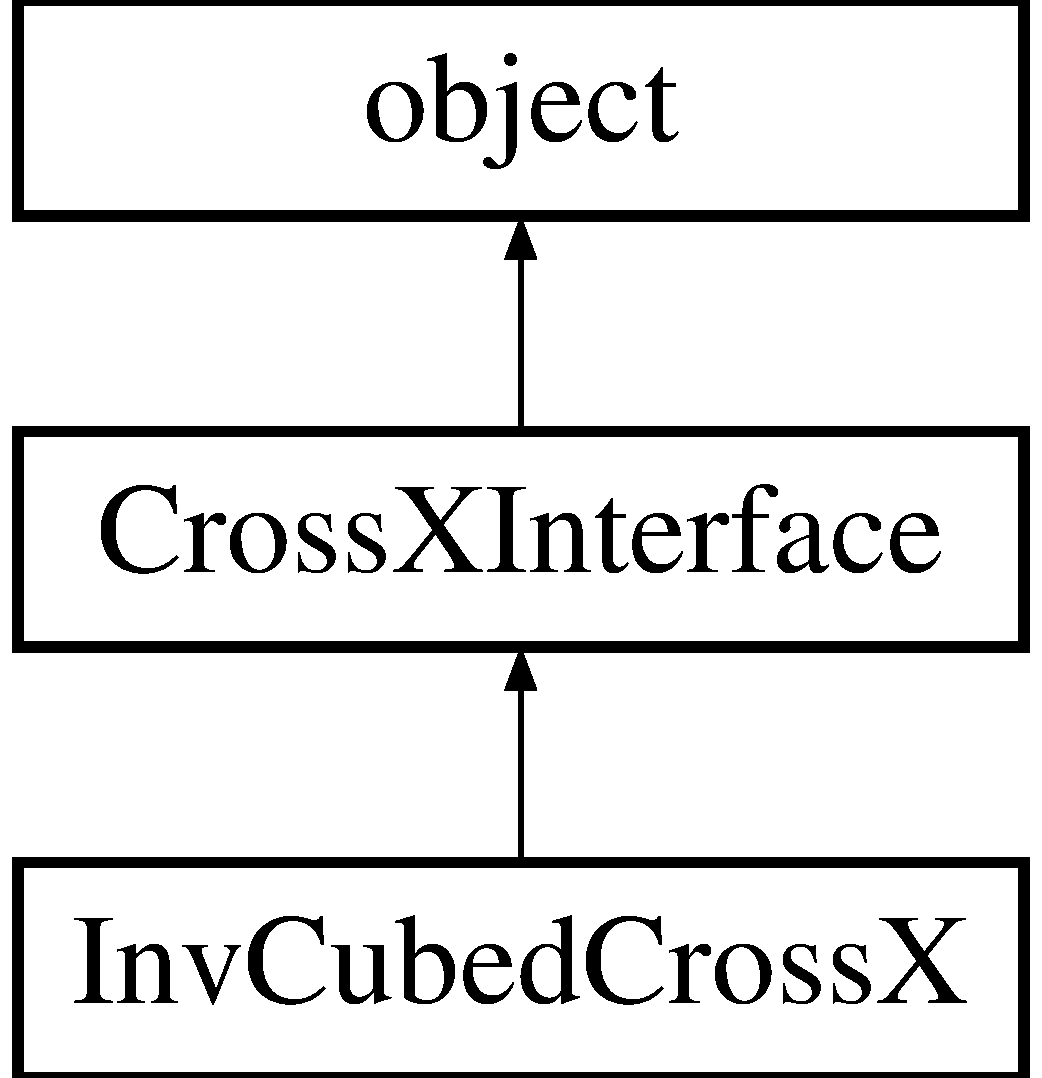
\includegraphics[height=3.000000cm]{classsrc_1_1_cross_x_interface_1_1_cross_x_interface}
\end{center}
\end{figure}
\subsection*{Public Member Functions}
\begin{DoxyCompactItemize}
\item 
def \hyperlink{classsrc_1_1_cross_x_interface_1_1_cross_x_interface_ac775ee34451fdfa742b318538164070e}{\-\_\-\-\_\-init\-\_\-\-\_\-}
\begin{DoxyCompactList}\small\item\em Constructor. \end{DoxyCompactList}\item 
def \hyperlink{classsrc_1_1_cross_x_interface_1_1_cross_x_interface_aa7a4b9bc0941308e362738503137460e}{\-\_\-\-\_\-str\-\_\-\-\_\-}
\begin{DoxyCompactList}\small\item\em Print string definition. \end{DoxyCompactList}\item 
def \hyperlink{classsrc_1_1_cross_x_interface_1_1_cross_x_interface_a738b60650d40ca81094acdae3cc55657}{update\-Cross\-X}
\begin{DoxyCompactList}\small\item\em Update function cross sections. \end{DoxyCompactList}\end{DoxyCompactItemize}
\subsection*{Public Attributes}
\begin{DoxyCompactItemize}
\item 
\hyperlink{classsrc_1_1_cross_x_interface_1_1_cross_x_interface_ab19871ffd067470950336cff88f8b1da}{sig\-\_\-a}
\begin{DoxyCompactList}\small\item\em $\sigma_a$, the absorption cross section \end{DoxyCompactList}\item 
\hyperlink{classsrc_1_1_cross_x_interface_1_1_cross_x_interface_afb10e3cd4777a9b381a31a32071fc0d1}{sig\-\_\-s}
\begin{DoxyCompactList}\small\item\em $\sigma_s$, the scattering cross section \end{DoxyCompactList}\item 
\hyperlink{classsrc_1_1_cross_x_interface_1_1_cross_x_interface_a9aa02ff48c273c3bc0a8213a045e6f4e}{sig\-\_\-t}
\begin{DoxyCompactList}\small\item\em $\sigma_t$, the total cross section \end{DoxyCompactList}\end{DoxyCompactItemize}


\subsection{Detailed Description}
Cross section class. 

Class that handles the cross sections at a particular point in space. If we want to make temperature dependent cross sections later, we will make a class that derives from this class. The derived class will have a function to update the need to change this later.

All Cross sections have units of $\mbox{cm}^{-1}$. The basic cross sections included by this class are $\sigma_t$, $\sigma_s$, and $\sigma_a$, where $\sigma_t = \sigma_s+\sigma_a$. 

\subsection{Constructor \& Destructor Documentation}
\hypertarget{classsrc_1_1_cross_x_interface_1_1_cross_x_interface_ac775ee34451fdfa742b318538164070e}{\index{src\-::\-Cross\-X\-Interface\-::\-Cross\-X\-Interface@{src\-::\-Cross\-X\-Interface\-::\-Cross\-X\-Interface}!\-\_\-\-\_\-init\-\_\-\-\_\-@{\-\_\-\-\_\-init\-\_\-\-\_\-}}
\index{\-\_\-\-\_\-init\-\_\-\-\_\-@{\-\_\-\-\_\-init\-\_\-\-\_\-}!src::CrossXInterface::CrossXInterface@{src\-::\-Cross\-X\-Interface\-::\-Cross\-X\-Interface}}
\subsubsection[{\-\_\-\-\_\-init\-\_\-\-\_\-}]{\setlength{\rightskip}{0pt plus 5cm}def \-\_\-\-\_\-init\-\_\-\-\_\- (
\begin{DoxyParamCaption}
\item[{}]{self, }
\item[{}]{sigma\-\_\-a, }
\item[{}]{sigma\-\_\-s}
\end{DoxyParamCaption}
)}}\label{classsrc_1_1_cross_x_interface_1_1_cross_x_interface_ac775ee34451fdfa742b318538164070e}


Constructor. 

Takes $\sigma_a$ and $\sigma_s$ and computes $\sigma_t$.


\begin{DoxyParams}[1]{Parameters}
\mbox{\tt in}  & {\em self} & self \\
\hline
\mbox{\tt in}  & {\em sigma\-\_\-a} & $\sigma_a$, the absorption cross section \\
\hline
\mbox{\tt in}  & {\em sigma\-\_\-s} & $\sigma_s$, the scattering cross section \\
\hline
\end{DoxyParams}


\subsection{Member Function Documentation}
\hypertarget{classsrc_1_1_cross_x_interface_1_1_cross_x_interface_aa7a4b9bc0941308e362738503137460e}{\index{src\-::\-Cross\-X\-Interface\-::\-Cross\-X\-Interface@{src\-::\-Cross\-X\-Interface\-::\-Cross\-X\-Interface}!\-\_\-\-\_\-str\-\_\-\-\_\-@{\-\_\-\-\_\-str\-\_\-\-\_\-}}
\index{\-\_\-\-\_\-str\-\_\-\-\_\-@{\-\_\-\-\_\-str\-\_\-\-\_\-}!src::CrossXInterface::CrossXInterface@{src\-::\-Cross\-X\-Interface\-::\-Cross\-X\-Interface}}
\subsubsection[{\-\_\-\-\_\-str\-\_\-\-\_\-}]{\setlength{\rightskip}{0pt plus 5cm}def \-\_\-\-\_\-str\-\_\-\-\_\- (
\begin{DoxyParamCaption}
\item[{}]{self}
\end{DoxyParamCaption}
)}}\label{classsrc_1_1_cross_x_interface_1_1_cross_x_interface_aa7a4b9bc0941308e362738503137460e}


Print string definition. 

Defines how to print the object. Prints $\sigma_s$, $\sigma_a$, and $\sigma_t$.


\begin{DoxyParams}[1]{Parameters}
\mbox{\tt in}  & {\em self} & self \\
\hline
\end{DoxyParams}
\begin{DoxyReturn}{Returns}
string to be printed with the print command 
\end{DoxyReturn}
\hypertarget{classsrc_1_1_cross_x_interface_1_1_cross_x_interface_a738b60650d40ca81094acdae3cc55657}{\index{src\-::\-Cross\-X\-Interface\-::\-Cross\-X\-Interface@{src\-::\-Cross\-X\-Interface\-::\-Cross\-X\-Interface}!update\-Cross\-X@{update\-Cross\-X}}
\index{update\-Cross\-X@{update\-Cross\-X}!src::CrossXInterface::CrossXInterface@{src\-::\-Cross\-X\-Interface\-::\-Cross\-X\-Interface}}
\subsubsection[{update\-Cross\-X}]{\setlength{\rightskip}{0pt plus 5cm}def update\-Cross\-X (
\begin{DoxyParamCaption}
\item[{}]{self, }
\item[{}]{args, }
\item[{}]{kwargs}
\end{DoxyParamCaption}
)}}\label{classsrc_1_1_cross_x_interface_1_1_cross_x_interface_a738b60650d40ca81094acdae3cc55657}


Update function cross sections. 

In this base class, cross sections are not updated by default; if it is necessary to update cross sections, this will be done by a derived class.


\begin{DoxyParams}[1]{Parameters}
\mbox{\tt in}  & {\em args} & arbitrary number of arguments \\
\hline
\mbox{\tt in}  & {\em kwargs} & arbitrary number of keyword arguments \\
\hline
\end{DoxyParams}


\subsection{Member Data Documentation}
\hypertarget{classsrc_1_1_cross_x_interface_1_1_cross_x_interface_ab19871ffd067470950336cff88f8b1da}{\index{src\-::\-Cross\-X\-Interface\-::\-Cross\-X\-Interface@{src\-::\-Cross\-X\-Interface\-::\-Cross\-X\-Interface}!sig\-\_\-a@{sig\-\_\-a}}
\index{sig\-\_\-a@{sig\-\_\-a}!src::CrossXInterface::CrossXInterface@{src\-::\-Cross\-X\-Interface\-::\-Cross\-X\-Interface}}
\subsubsection[{sig\-\_\-a}]{\setlength{\rightskip}{0pt plus 5cm}sig\-\_\-a}}\label{classsrc_1_1_cross_x_interface_1_1_cross_x_interface_ab19871ffd067470950336cff88f8b1da}


$\sigma_a$, the absorption cross section 

\hypertarget{classsrc_1_1_cross_x_interface_1_1_cross_x_interface_afb10e3cd4777a9b381a31a32071fc0d1}{\index{src\-::\-Cross\-X\-Interface\-::\-Cross\-X\-Interface@{src\-::\-Cross\-X\-Interface\-::\-Cross\-X\-Interface}!sig\-\_\-s@{sig\-\_\-s}}
\index{sig\-\_\-s@{sig\-\_\-s}!src::CrossXInterface::CrossXInterface@{src\-::\-Cross\-X\-Interface\-::\-Cross\-X\-Interface}}
\subsubsection[{sig\-\_\-s}]{\setlength{\rightskip}{0pt plus 5cm}sig\-\_\-s}}\label{classsrc_1_1_cross_x_interface_1_1_cross_x_interface_afb10e3cd4777a9b381a31a32071fc0d1}


$\sigma_s$, the scattering cross section 

\hypertarget{classsrc_1_1_cross_x_interface_1_1_cross_x_interface_a9aa02ff48c273c3bc0a8213a045e6f4e}{\index{src\-::\-Cross\-X\-Interface\-::\-Cross\-X\-Interface@{src\-::\-Cross\-X\-Interface\-::\-Cross\-X\-Interface}!sig\-\_\-t@{sig\-\_\-t}}
\index{sig\-\_\-t@{sig\-\_\-t}!src::CrossXInterface::CrossXInterface@{src\-::\-Cross\-X\-Interface\-::\-Cross\-X\-Interface}}
\subsubsection[{sig\-\_\-t}]{\setlength{\rightskip}{0pt plus 5cm}sig\-\_\-t}}\label{classsrc_1_1_cross_x_interface_1_1_cross_x_interface_a9aa02ff48c273c3bc0a8213a045e6f4e}


$\sigma_t$, the total cross section 



The documentation for this class was generated from the following file\-:\begin{DoxyCompactItemize}
\item 
src/\hyperlink{_cross_x_interface_8py}{Cross\-X\-Interface.\-py}\end{DoxyCompactItemize}

\hypertarget{classsrc_1_1_mesh_1_1_element}{\section{Element Class Reference}
\label{classsrc_1_1_mesh_1_1_element}\index{Element@{Element}}
}
\subsection*{Public Member Functions}
\begin{DoxyCompactItemize}
\item 
def \hyperlink{classsrc_1_1_mesh_1_1_element_ac775ee34451fdfa742b318538164070e}{\-\_\-\-\_\-init\-\_\-\-\_\-}
\begin{DoxyCompactList}\small\item\em Simple constructor. \end{DoxyCompactList}\item 
def \hyperlink{classsrc_1_1_mesh_1_1_element_aa7a4b9bc0941308e362738503137460e}{\-\_\-\-\_\-str\-\_\-\-\_\-}
\end{DoxyCompactItemize}
\subsection*{Public Attributes}
\begin{DoxyCompactItemize}
\item 
\hyperlink{classsrc_1_1_mesh_1_1_element_aacddc911cdfe5cd5ec97b084754542d4}{dx}
\item 
\hyperlink{classsrc_1_1_mesh_1_1_element_ae6d1f7a1542ce73d6d9913c97961d5ea}{el\-\_\-id}
\item 
\hyperlink{classsrc_1_1_mesh_1_1_element_accf6c197a418ed2d049c5648d9c71a9e}{x\-\_\-cent}
\item 
\hyperlink{classsrc_1_1_mesh_1_1_element_a3c53fbdcb4e4034433f7fb548430436d}{xl}
\item 
\hyperlink{classsrc_1_1_mesh_1_1_element_a67ac9cf4961c762581641460beb3d936}{xr}
\end{DoxyCompactItemize}


\subsection{Constructor \& Destructor Documentation}
\hypertarget{classsrc_1_1_mesh_1_1_element_ac775ee34451fdfa742b318538164070e}{\index{src\-::\-Mesh\-::\-Element@{src\-::\-Mesh\-::\-Element}!\-\_\-\-\_\-init\-\_\-\-\_\-@{\-\_\-\-\_\-init\-\_\-\-\_\-}}
\index{\-\_\-\-\_\-init\-\_\-\-\_\-@{\-\_\-\-\_\-init\-\_\-\-\_\-}!src::Mesh::Element@{src\-::\-Mesh\-::\-Element}}
\subsubsection[{\-\_\-\-\_\-init\-\_\-\-\_\-}]{\setlength{\rightskip}{0pt plus 5cm}def \-\_\-\-\_\-init\-\_\-\-\_\- (
\begin{DoxyParamCaption}
\item[{}]{self, }
\item[{}]{el\-\_\-id, }
\item[{}]{x\-\_\-center, }
\item[{}]{width}
\end{DoxyParamCaption}
)}}\label{classsrc_1_1_mesh_1_1_element_ac775ee34451fdfa742b318538164070e}


Simple constructor. 

Takes in I\-D, center, and width of element 

\subsection{Member Function Documentation}
\hypertarget{classsrc_1_1_mesh_1_1_element_aa7a4b9bc0941308e362738503137460e}{\index{src\-::\-Mesh\-::\-Element@{src\-::\-Mesh\-::\-Element}!\-\_\-\-\_\-str\-\_\-\-\_\-@{\-\_\-\-\_\-str\-\_\-\-\_\-}}
\index{\-\_\-\-\_\-str\-\_\-\-\_\-@{\-\_\-\-\_\-str\-\_\-\-\_\-}!src::Mesh::Element@{src\-::\-Mesh\-::\-Element}}
\subsubsection[{\-\_\-\-\_\-str\-\_\-\-\_\-}]{\setlength{\rightskip}{0pt plus 5cm}def \-\_\-\-\_\-str\-\_\-\-\_\- (
\begin{DoxyParamCaption}
\item[{}]{self}
\end{DoxyParamCaption}
)}}\label{classsrc_1_1_mesh_1_1_element_aa7a4b9bc0941308e362738503137460e}


\subsection{Member Data Documentation}
\hypertarget{classsrc_1_1_mesh_1_1_element_aacddc911cdfe5cd5ec97b084754542d4}{\index{src\-::\-Mesh\-::\-Element@{src\-::\-Mesh\-::\-Element}!dx@{dx}}
\index{dx@{dx}!src::Mesh::Element@{src\-::\-Mesh\-::\-Element}}
\subsubsection[{dx}]{\setlength{\rightskip}{0pt plus 5cm}dx}}\label{classsrc_1_1_mesh_1_1_element_aacddc911cdfe5cd5ec97b084754542d4}
\hypertarget{classsrc_1_1_mesh_1_1_element_ae6d1f7a1542ce73d6d9913c97961d5ea}{\index{src\-::\-Mesh\-::\-Element@{src\-::\-Mesh\-::\-Element}!el\-\_\-id@{el\-\_\-id}}
\index{el\-\_\-id@{el\-\_\-id}!src::Mesh::Element@{src\-::\-Mesh\-::\-Element}}
\subsubsection[{el\-\_\-id}]{\setlength{\rightskip}{0pt plus 5cm}el\-\_\-id}}\label{classsrc_1_1_mesh_1_1_element_ae6d1f7a1542ce73d6d9913c97961d5ea}
\hypertarget{classsrc_1_1_mesh_1_1_element_accf6c197a418ed2d049c5648d9c71a9e}{\index{src\-::\-Mesh\-::\-Element@{src\-::\-Mesh\-::\-Element}!x\-\_\-cent@{x\-\_\-cent}}
\index{x\-\_\-cent@{x\-\_\-cent}!src::Mesh::Element@{src\-::\-Mesh\-::\-Element}}
\subsubsection[{x\-\_\-cent}]{\setlength{\rightskip}{0pt plus 5cm}x\-\_\-cent}}\label{classsrc_1_1_mesh_1_1_element_accf6c197a418ed2d049c5648d9c71a9e}
\hypertarget{classsrc_1_1_mesh_1_1_element_a3c53fbdcb4e4034433f7fb548430436d}{\index{src\-::\-Mesh\-::\-Element@{src\-::\-Mesh\-::\-Element}!xl@{xl}}
\index{xl@{xl}!src::Mesh::Element@{src\-::\-Mesh\-::\-Element}}
\subsubsection[{xl}]{\setlength{\rightskip}{0pt plus 5cm}xl}}\label{classsrc_1_1_mesh_1_1_element_a3c53fbdcb4e4034433f7fb548430436d}
\hypertarget{classsrc_1_1_mesh_1_1_element_a67ac9cf4961c762581641460beb3d936}{\index{src\-::\-Mesh\-::\-Element@{src\-::\-Mesh\-::\-Element}!xr@{xr}}
\index{xr@{xr}!src::Mesh::Element@{src\-::\-Mesh\-::\-Element}}
\subsubsection[{xr}]{\setlength{\rightskip}{0pt plus 5cm}xr}}\label{classsrc_1_1_mesh_1_1_element_a67ac9cf4961c762581641460beb3d936}


The documentation for this class was generated from the following file\-:\begin{DoxyCompactItemize}
\item 
src/\hyperlink{_mesh_8py}{Mesh.\-py}\end{DoxyCompactItemize}

\hypertarget{classsrc_1_1_muscl_hanc_1_1_hydro_state}{\section{Hydro\-State Class Reference}
\label{classsrc_1_1_muscl_hanc_1_1_hydro_state}\index{Hydro\-State@{Hydro\-State}}
}
\subsection*{Public Member Functions}
\begin{DoxyCompactItemize}
\item 
def \hyperlink{classsrc_1_1_muscl_hanc_1_1_hydro_state_ac775ee34451fdfa742b318538164070e}{\-\_\-\-\_\-init\-\_\-\-\_\-}
\item 
def \hyperlink{classsrc_1_1_muscl_hanc_1_1_hydro_state_a449f8fd74d358c0ad641b6c6d6917ba0}{\-\_\-\-\_\-eq\-\_\-\-\_\-}
\item 
def \hyperlink{classsrc_1_1_muscl_hanc_1_1_hydro_state_aa7a4b9bc0941308e362738503137460e}{\-\_\-\-\_\-str\-\_\-\-\_\-}
\item 
def \hyperlink{classsrc_1_1_muscl_hanc_1_1_hydro_state_aaaef2d0d9f0d8ae2018f145248ffcf8f}{get\-Sound\-Speed}
\item 
def \hyperlink{classsrc_1_1_muscl_hanc_1_1_hydro_state_a5bcd76e987be8143f8a814c7d47276ff}{update\-State}
\end{DoxyCompactItemize}
\subsection*{Public Attributes}
\begin{DoxyCompactItemize}
\item 
\hyperlink{classsrc_1_1_muscl_hanc_1_1_hydro_state_a08a4415e9d594ff960030b921d42b91e}{e}
\item 
\hyperlink{classsrc_1_1_muscl_hanc_1_1_hydro_state_a8d00631c9622112f1877fdb1222c242e}{gamma}
\item 
\hyperlink{classsrc_1_1_muscl_hanc_1_1_hydro_state_ac483f6ce851c9ecd9fb835ff7551737c}{p}
\item 
\hyperlink{classsrc_1_1_muscl_hanc_1_1_hydro_state_ab8ec92cc3ea8422c9349409bae98d2a0}{rho}
\item 
\hyperlink{classsrc_1_1_muscl_hanc_1_1_hydro_state_a6277e2a7446059985dc9bcf0a4ac1a8f}{u}
\end{DoxyCompactItemize}
\subsection*{Private Attributes}
\begin{DoxyCompactItemize}
\item 
\hyperlink{classsrc_1_1_muscl_hanc_1_1_hydro_state_ae55534cfed72fbc20108277a88fdc073}{\-\_\-\-\_\-dict\-\_\-\-\_\-}
\end{DoxyCompactItemize}


\subsection{Constructor \& Destructor Documentation}
\hypertarget{classsrc_1_1_muscl_hanc_1_1_hydro_state_ac775ee34451fdfa742b318538164070e}{\index{src\-::\-Muscl\-Hanc\-::\-Hydro\-State@{src\-::\-Muscl\-Hanc\-::\-Hydro\-State}!\-\_\-\-\_\-init\-\_\-\-\_\-@{\-\_\-\-\_\-init\-\_\-\-\_\-}}
\index{\-\_\-\-\_\-init\-\_\-\-\_\-@{\-\_\-\-\_\-init\-\_\-\-\_\-}!src::MusclHanc::HydroState@{src\-::\-Muscl\-Hanc\-::\-Hydro\-State}}
\subsubsection[{\-\_\-\-\_\-init\-\_\-\-\_\-}]{\setlength{\rightskip}{0pt plus 5cm}def \-\_\-\-\_\-init\-\_\-\-\_\- (
\begin{DoxyParamCaption}
\item[{}]{self, }
\item[{}]{u = {\ttfamily None}, }
\item[{}]{rho = {\ttfamily None}, }
\item[{}]{p = {\ttfamily None}, }
\item[{}]{gamma = {\ttfamily None}}
\end{DoxyParamCaption}
)}}\label{classsrc_1_1_muscl_hanc_1_1_hydro_state_ac775ee34451fdfa742b318538164070e}


\subsection{Member Function Documentation}
\hypertarget{classsrc_1_1_muscl_hanc_1_1_hydro_state_a449f8fd74d358c0ad641b6c6d6917ba0}{\index{src\-::\-Muscl\-Hanc\-::\-Hydro\-State@{src\-::\-Muscl\-Hanc\-::\-Hydro\-State}!\-\_\-\-\_\-eq\-\_\-\-\_\-@{\-\_\-\-\_\-eq\-\_\-\-\_\-}}
\index{\-\_\-\-\_\-eq\-\_\-\-\_\-@{\-\_\-\-\_\-eq\-\_\-\-\_\-}!src::MusclHanc::HydroState@{src\-::\-Muscl\-Hanc\-::\-Hydro\-State}}
\subsubsection[{\-\_\-\-\_\-eq\-\_\-\-\_\-}]{\setlength{\rightskip}{0pt plus 5cm}def \-\_\-\-\_\-eq\-\_\-\-\_\- (
\begin{DoxyParamCaption}
\item[{}]{self, }
\item[{}]{other}
\end{DoxyParamCaption}
)}}\label{classsrc_1_1_muscl_hanc_1_1_hydro_state_a449f8fd74d358c0ad641b6c6d6917ba0}
\hypertarget{classsrc_1_1_muscl_hanc_1_1_hydro_state_aa7a4b9bc0941308e362738503137460e}{\index{src\-::\-Muscl\-Hanc\-::\-Hydro\-State@{src\-::\-Muscl\-Hanc\-::\-Hydro\-State}!\-\_\-\-\_\-str\-\_\-\-\_\-@{\-\_\-\-\_\-str\-\_\-\-\_\-}}
\index{\-\_\-\-\_\-str\-\_\-\-\_\-@{\-\_\-\-\_\-str\-\_\-\-\_\-}!src::MusclHanc::HydroState@{src\-::\-Muscl\-Hanc\-::\-Hydro\-State}}
\subsubsection[{\-\_\-\-\_\-str\-\_\-\-\_\-}]{\setlength{\rightskip}{0pt plus 5cm}def \-\_\-\-\_\-str\-\_\-\-\_\- (
\begin{DoxyParamCaption}
\item[{}]{self}
\end{DoxyParamCaption}
)}}\label{classsrc_1_1_muscl_hanc_1_1_hydro_state_aa7a4b9bc0941308e362738503137460e}
\hypertarget{classsrc_1_1_muscl_hanc_1_1_hydro_state_aaaef2d0d9f0d8ae2018f145248ffcf8f}{\index{src\-::\-Muscl\-Hanc\-::\-Hydro\-State@{src\-::\-Muscl\-Hanc\-::\-Hydro\-State}!get\-Sound\-Speed@{get\-Sound\-Speed}}
\index{get\-Sound\-Speed@{get\-Sound\-Speed}!src::MusclHanc::HydroState@{src\-::\-Muscl\-Hanc\-::\-Hydro\-State}}
\subsubsection[{get\-Sound\-Speed}]{\setlength{\rightskip}{0pt plus 5cm}def get\-Sound\-Speed (
\begin{DoxyParamCaption}
\item[{}]{self}
\end{DoxyParamCaption}
)}}\label{classsrc_1_1_muscl_hanc_1_1_hydro_state_aaaef2d0d9f0d8ae2018f145248ffcf8f}
\hypertarget{classsrc_1_1_muscl_hanc_1_1_hydro_state_a5bcd76e987be8143f8a814c7d47276ff}{\index{src\-::\-Muscl\-Hanc\-::\-Hydro\-State@{src\-::\-Muscl\-Hanc\-::\-Hydro\-State}!update\-State@{update\-State}}
\index{update\-State@{update\-State}!src::MusclHanc::HydroState@{src\-::\-Muscl\-Hanc\-::\-Hydro\-State}}
\subsubsection[{update\-State}]{\setlength{\rightskip}{0pt plus 5cm}def update\-State (
\begin{DoxyParamCaption}
\item[{}]{self, }
\item[{}]{rho, }
\item[{}]{mom, }
\item[{}]{erg}
\end{DoxyParamCaption}
)}}\label{classsrc_1_1_muscl_hanc_1_1_hydro_state_a5bcd76e987be8143f8a814c7d47276ff}


\subsection{Member Data Documentation}
\hypertarget{classsrc_1_1_muscl_hanc_1_1_hydro_state_ae55534cfed72fbc20108277a88fdc073}{\index{src\-::\-Muscl\-Hanc\-::\-Hydro\-State@{src\-::\-Muscl\-Hanc\-::\-Hydro\-State}!\-\_\-\-\_\-dict\-\_\-\-\_\-@{\-\_\-\-\_\-dict\-\_\-\-\_\-}}
\index{\-\_\-\-\_\-dict\-\_\-\-\_\-@{\-\_\-\-\_\-dict\-\_\-\-\_\-}!src::MusclHanc::HydroState@{src\-::\-Muscl\-Hanc\-::\-Hydro\-State}}
\subsubsection[{\-\_\-\-\_\-dict\-\_\-\-\_\-}]{\setlength{\rightskip}{0pt plus 5cm}\-\_\-\-\_\-dict\-\_\-\-\_\-\hspace{0.3cm}{\ttfamily [private]}}}\label{classsrc_1_1_muscl_hanc_1_1_hydro_state_ae55534cfed72fbc20108277a88fdc073}
\hypertarget{classsrc_1_1_muscl_hanc_1_1_hydro_state_a08a4415e9d594ff960030b921d42b91e}{\index{src\-::\-Muscl\-Hanc\-::\-Hydro\-State@{src\-::\-Muscl\-Hanc\-::\-Hydro\-State}!e@{e}}
\index{e@{e}!src::MusclHanc::HydroState@{src\-::\-Muscl\-Hanc\-::\-Hydro\-State}}
\subsubsection[{e}]{\setlength{\rightskip}{0pt plus 5cm}e}}\label{classsrc_1_1_muscl_hanc_1_1_hydro_state_a08a4415e9d594ff960030b921d42b91e}
\hypertarget{classsrc_1_1_muscl_hanc_1_1_hydro_state_a8d00631c9622112f1877fdb1222c242e}{\index{src\-::\-Muscl\-Hanc\-::\-Hydro\-State@{src\-::\-Muscl\-Hanc\-::\-Hydro\-State}!gamma@{gamma}}
\index{gamma@{gamma}!src::MusclHanc::HydroState@{src\-::\-Muscl\-Hanc\-::\-Hydro\-State}}
\subsubsection[{gamma}]{\setlength{\rightskip}{0pt plus 5cm}gamma}}\label{classsrc_1_1_muscl_hanc_1_1_hydro_state_a8d00631c9622112f1877fdb1222c242e}
\hypertarget{classsrc_1_1_muscl_hanc_1_1_hydro_state_ac483f6ce851c9ecd9fb835ff7551737c}{\index{src\-::\-Muscl\-Hanc\-::\-Hydro\-State@{src\-::\-Muscl\-Hanc\-::\-Hydro\-State}!p@{p}}
\index{p@{p}!src::MusclHanc::HydroState@{src\-::\-Muscl\-Hanc\-::\-Hydro\-State}}
\subsubsection[{p}]{\setlength{\rightskip}{0pt plus 5cm}p}}\label{classsrc_1_1_muscl_hanc_1_1_hydro_state_ac483f6ce851c9ecd9fb835ff7551737c}
\hypertarget{classsrc_1_1_muscl_hanc_1_1_hydro_state_ab8ec92cc3ea8422c9349409bae98d2a0}{\index{src\-::\-Muscl\-Hanc\-::\-Hydro\-State@{src\-::\-Muscl\-Hanc\-::\-Hydro\-State}!rho@{rho}}
\index{rho@{rho}!src::MusclHanc::HydroState@{src\-::\-Muscl\-Hanc\-::\-Hydro\-State}}
\subsubsection[{rho}]{\setlength{\rightskip}{0pt plus 5cm}rho}}\label{classsrc_1_1_muscl_hanc_1_1_hydro_state_ab8ec92cc3ea8422c9349409bae98d2a0}
\hypertarget{classsrc_1_1_muscl_hanc_1_1_hydro_state_a6277e2a7446059985dc9bcf0a4ac1a8f}{\index{src\-::\-Muscl\-Hanc\-::\-Hydro\-State@{src\-::\-Muscl\-Hanc\-::\-Hydro\-State}!u@{u}}
\index{u@{u}!src::MusclHanc::HydroState@{src\-::\-Muscl\-Hanc\-::\-Hydro\-State}}
\subsubsection[{u}]{\setlength{\rightskip}{0pt plus 5cm}u}}\label{classsrc_1_1_muscl_hanc_1_1_hydro_state_a6277e2a7446059985dc9bcf0a4ac1a8f}


The documentation for this class was generated from the following file\-:\begin{DoxyCompactItemize}
\item 
src/\hyperlink{_muscl_hanc_8py}{Muscl\-Hanc.\-py}\end{DoxyCompactItemize}

\hypertarget{classsrc_1_1_cross_x_interface_1_1_inv_cubed_cross_x}{\section{Inv\-Cubed\-Cross\-X Class Reference}
\label{classsrc_1_1_cross_x_interface_1_1_inv_cubed_cross_x}\index{Inv\-Cubed\-Cross\-X@{Inv\-Cubed\-Cross\-X}}
}


Inverse cubed cross section class.  


Inheritance diagram for Inv\-Cubed\-Cross\-X\-:\begin{figure}[H]
\begin{center}
\leavevmode
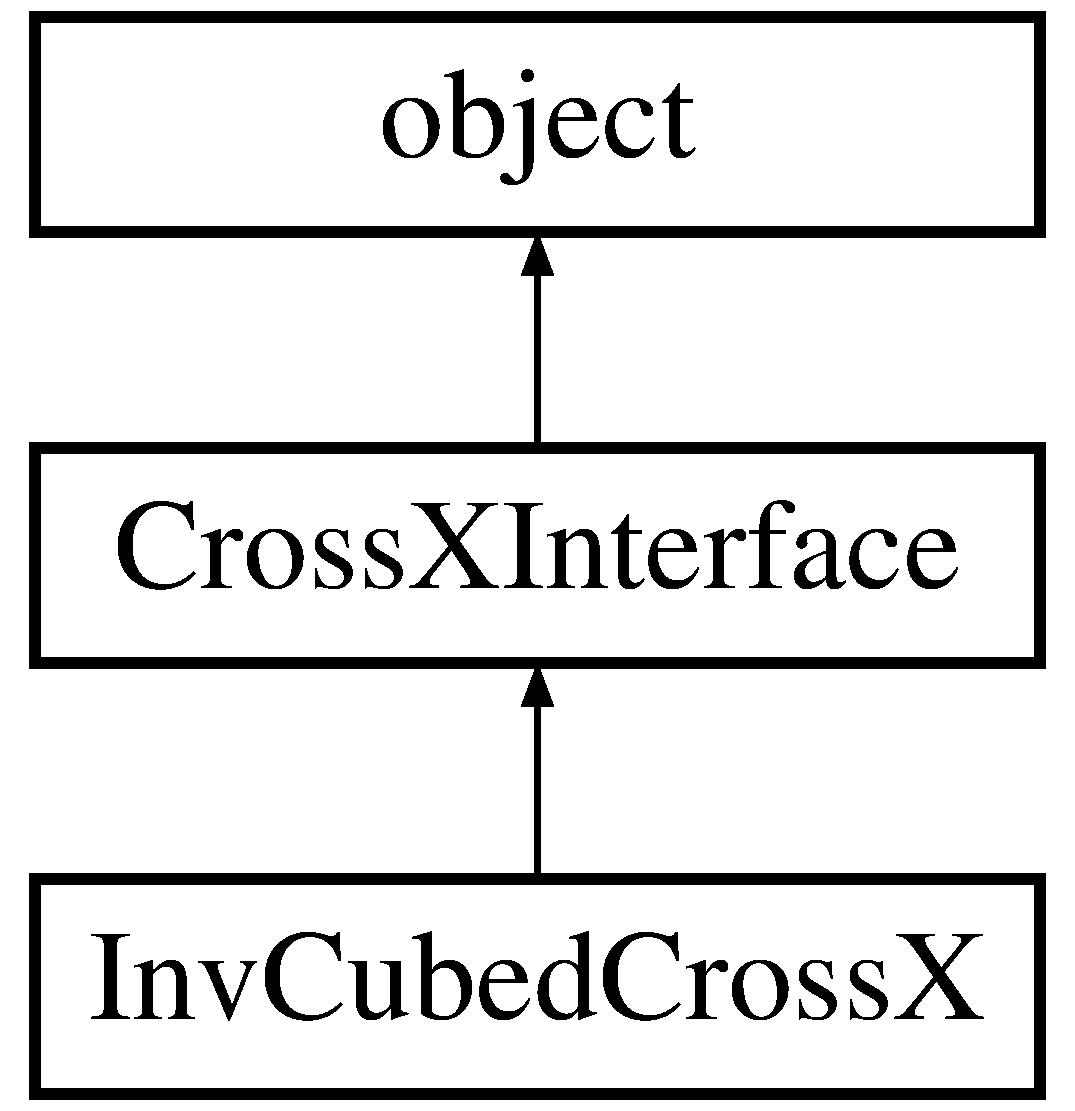
\includegraphics[height=3.000000cm]{classsrc_1_1_cross_x_interface_1_1_inv_cubed_cross_x}
\end{center}
\end{figure}
\subsection*{Public Member Functions}
\begin{DoxyCompactItemize}
\item 
def \hyperlink{classsrc_1_1_cross_x_interface_1_1_inv_cubed_cross_x_ac775ee34451fdfa742b318538164070e}{\-\_\-\-\_\-init\-\_\-\-\_\-}
\begin{DoxyCompactList}\small\item\em Constructor. \end{DoxyCompactList}\item 
def \hyperlink{classsrc_1_1_cross_x_interface_1_1_inv_cubed_cross_x_a738b60650d40ca81094acdae3cc55657}{update\-Cross\-X}
\begin{DoxyCompactList}\small\item\em Update function for cross sections. \end{DoxyCompactList}\end{DoxyCompactItemize}
\subsection*{Public Attributes}
\begin{DoxyCompactItemize}
\item 
\hyperlink{classsrc_1_1_cross_x_interface_1_1_inv_cubed_cross_x_a683c89e90662ba53f43be1061d4e39aa}{coeff}
\begin{DoxyCompactList}\small\item\em scale coefficient $c_a$ in $\sigma_a = c_a \rho T^{-3}$ \end{DoxyCompactList}\item 
\hyperlink{classsrc_1_1_cross_x_interface_1_1_inv_cubed_cross_x_ab19871ffd067470950336cff88f8b1da}{sig\-\_\-a}
\item 
\hyperlink{classsrc_1_1_cross_x_interface_1_1_inv_cubed_cross_x_afb10e3cd4777a9b381a31a32071fc0d1}{sig\-\_\-s}
\item 
\hyperlink{classsrc_1_1_cross_x_interface_1_1_inv_cubed_cross_x_a9aa02ff48c273c3bc0a8213a045e6f4e}{sig\-\_\-t}
\end{DoxyCompactItemize}


\subsection{Detailed Description}
Inverse cubed cross section class. 

\hyperlink{namespace_this}{This} is an example of a derived cross section. In this case it is a simple Inv\-Cubed relation where you need to pass in a new density and temperature to update the cross section. Anything that uses the base class should be able to interact with base class objects.

These cross sections are computed as

\[ \sigma_s = \sigma_s^{'''} \rho \] \[ \sigma_a = c_a \rho T^{-3} \] 

\subsection{Constructor \& Destructor Documentation}
\hypertarget{classsrc_1_1_cross_x_interface_1_1_inv_cubed_cross_x_ac775ee34451fdfa742b318538164070e}{\index{src\-::\-Cross\-X\-Interface\-::\-Inv\-Cubed\-Cross\-X@{src\-::\-Cross\-X\-Interface\-::\-Inv\-Cubed\-Cross\-X}!\-\_\-\-\_\-init\-\_\-\-\_\-@{\-\_\-\-\_\-init\-\_\-\-\_\-}}
\index{\-\_\-\-\_\-init\-\_\-\-\_\-@{\-\_\-\-\_\-init\-\_\-\-\_\-}!src::CrossXInterface::InvCubedCrossX@{src\-::\-Cross\-X\-Interface\-::\-Inv\-Cubed\-Cross\-X}}
\subsubsection[{\-\_\-\-\_\-init\-\_\-\-\_\-}]{\setlength{\rightskip}{0pt plus 5cm}def \-\_\-\-\_\-init\-\_\-\-\_\- (
\begin{DoxyParamCaption}
\item[{}]{self, }
\item[{}]{sigma\-\_\-s\-\_\-micro, }
\item[{}]{rho, }
\item[{}]{temp, }
\item[{}]{scale\-\_\-coeff = {\ttfamily 1.0}}
\end{DoxyParamCaption}
)}}\label{classsrc_1_1_cross_x_interface_1_1_inv_cubed_cross_x_ac775ee34451fdfa742b318538164070e}


Constructor. 

Takes the micro scattering cross section, density, temperature, and scaling coefficient and computes cross sections.


\begin{DoxyParams}[1]{Parameters}
\mbox{\tt in}  & {\em self} & self \\
\hline
\mbox{\tt in}  & {\em sigma\-\_\-s\-\_\-micro} & $\sigma_s^{'''}$, the micro scattering cross section, equal to $\frac{\sigma_s}{\rho}$ \\
\hline
\mbox{\tt in}  & {\em rho} & $\rho$, density \\
\hline
\mbox{\tt in}  & {\em temp} & $T$, temperature \\
\hline
\mbox{\tt in}  & {\em scale\-\_\-coeff} & $c_a$, the scale coefficient in $\sigma_a = c_a \rho T^{-3}$ \\
\hline
\end{DoxyParams}


\subsection{Member Function Documentation}
\hypertarget{classsrc_1_1_cross_x_interface_1_1_inv_cubed_cross_x_a738b60650d40ca81094acdae3cc55657}{\index{src\-::\-Cross\-X\-Interface\-::\-Inv\-Cubed\-Cross\-X@{src\-::\-Cross\-X\-Interface\-::\-Inv\-Cubed\-Cross\-X}!update\-Cross\-X@{update\-Cross\-X}}
\index{update\-Cross\-X@{update\-Cross\-X}!src::CrossXInterface::InvCubedCrossX@{src\-::\-Cross\-X\-Interface\-::\-Inv\-Cubed\-Cross\-X}}
\subsubsection[{update\-Cross\-X}]{\setlength{\rightskip}{0pt plus 5cm}def update\-Cross\-X (
\begin{DoxyParamCaption}
\item[{}]{self, }
\item[{}]{rho, }
\item[{}]{temp}
\end{DoxyParamCaption}
)}}\label{classsrc_1_1_cross_x_interface_1_1_inv_cubed_cross_x_a738b60650d40ca81094acdae3cc55657}


Update function for cross sections. 


\begin{DoxyParams}[1]{Parameters}
\mbox{\tt in}  & {\em self} & self \\
\hline
\mbox{\tt in}  & {\em rho} & $\rho$, density \\
\hline
\mbox{\tt in}  & {\em temp} & $T$, temperature \\
\hline
\end{DoxyParams}


\subsection{Member Data Documentation}
\hypertarget{classsrc_1_1_cross_x_interface_1_1_inv_cubed_cross_x_a683c89e90662ba53f43be1061d4e39aa}{\index{src\-::\-Cross\-X\-Interface\-::\-Inv\-Cubed\-Cross\-X@{src\-::\-Cross\-X\-Interface\-::\-Inv\-Cubed\-Cross\-X}!coeff@{coeff}}
\index{coeff@{coeff}!src::CrossXInterface::InvCubedCrossX@{src\-::\-Cross\-X\-Interface\-::\-Inv\-Cubed\-Cross\-X}}
\subsubsection[{coeff}]{\setlength{\rightskip}{0pt plus 5cm}coeff}}\label{classsrc_1_1_cross_x_interface_1_1_inv_cubed_cross_x_a683c89e90662ba53f43be1061d4e39aa}


scale coefficient $c_a$ in $\sigma_a = c_a \rho T^{-3}$ 

\hypertarget{classsrc_1_1_cross_x_interface_1_1_inv_cubed_cross_x_ab19871ffd067470950336cff88f8b1da}{\index{src\-::\-Cross\-X\-Interface\-::\-Inv\-Cubed\-Cross\-X@{src\-::\-Cross\-X\-Interface\-::\-Inv\-Cubed\-Cross\-X}!sig\-\_\-a@{sig\-\_\-a}}
\index{sig\-\_\-a@{sig\-\_\-a}!src::CrossXInterface::InvCubedCrossX@{src\-::\-Cross\-X\-Interface\-::\-Inv\-Cubed\-Cross\-X}}
\subsubsection[{sig\-\_\-a}]{\setlength{\rightskip}{0pt plus 5cm}sig\-\_\-a}}\label{classsrc_1_1_cross_x_interface_1_1_inv_cubed_cross_x_ab19871ffd067470950336cff88f8b1da}
\hypertarget{classsrc_1_1_cross_x_interface_1_1_inv_cubed_cross_x_afb10e3cd4777a9b381a31a32071fc0d1}{\index{src\-::\-Cross\-X\-Interface\-::\-Inv\-Cubed\-Cross\-X@{src\-::\-Cross\-X\-Interface\-::\-Inv\-Cubed\-Cross\-X}!sig\-\_\-s@{sig\-\_\-s}}
\index{sig\-\_\-s@{sig\-\_\-s}!src::CrossXInterface::InvCubedCrossX@{src\-::\-Cross\-X\-Interface\-::\-Inv\-Cubed\-Cross\-X}}
\subsubsection[{sig\-\_\-s}]{\setlength{\rightskip}{0pt plus 5cm}sig\-\_\-s}}\label{classsrc_1_1_cross_x_interface_1_1_inv_cubed_cross_x_afb10e3cd4777a9b381a31a32071fc0d1}
\hypertarget{classsrc_1_1_cross_x_interface_1_1_inv_cubed_cross_x_a9aa02ff48c273c3bc0a8213a045e6f4e}{\index{src\-::\-Cross\-X\-Interface\-::\-Inv\-Cubed\-Cross\-X@{src\-::\-Cross\-X\-Interface\-::\-Inv\-Cubed\-Cross\-X}!sig\-\_\-t@{sig\-\_\-t}}
\index{sig\-\_\-t@{sig\-\_\-t}!src::CrossXInterface::InvCubedCrossX@{src\-::\-Cross\-X\-Interface\-::\-Inv\-Cubed\-Cross\-X}}
\subsubsection[{sig\-\_\-t}]{\setlength{\rightskip}{0pt plus 5cm}sig\-\_\-t}}\label{classsrc_1_1_cross_x_interface_1_1_inv_cubed_cross_x_a9aa02ff48c273c3bc0a8213a045e6f4e}


The documentation for this class was generated from the following file\-:\begin{DoxyCompactItemize}
\item 
src/\hyperlink{_cross_x_interface_8py}{Cross\-X\-Interface.\-py}\end{DoxyCompactItemize}

\hypertarget{classsrc_1_1_mesh_1_1_mesh}{\section{Mesh Class Reference}
\label{classsrc_1_1_mesh_1_1_mesh}\index{Mesh@{Mesh}}
}


Class for mesh.  


\subsection*{Public Member Functions}
\begin{DoxyCompactItemize}
\item 
def \hyperlink{classsrc_1_1_mesh_1_1_mesh_ac775ee34451fdfa742b318538164070e}{\-\_\-\-\_\-init\-\_\-\-\_\-}
\item 
def \hyperlink{classsrc_1_1_mesh_1_1_mesh_aa7a4b9bc0941308e362738503137460e}{\-\_\-\-\_\-str\-\_\-\-\_\-}
\item 
def \hyperlink{classsrc_1_1_mesh_1_1_mesh_ae1fb639aa4d03c92c77dfdfab0ee2740}{get\-Element}
\end{DoxyCompactItemize}
\subsection*{Public Attributes}
\begin{DoxyCompactItemize}
\item 
\hyperlink{classsrc_1_1_mesh_1_1_mesh_aa9aaa650bacb9b91c82437c2ce48f50c}{elements}
\item 
\hyperlink{classsrc_1_1_mesh_1_1_mesh_ac31c5f98a6c4c5374dc0de3dad36e81e}{n\-\_\-elems}
\begin{DoxyCompactList}\small\item\em The mesh currently has fixed element widths, but let each element have one. \end{DoxyCompactList}\end{DoxyCompactItemize}


\subsection{Detailed Description}
Class for mesh. 

Just contains a list of element objects. \begin{DoxyVerb}Define the constructor. Pass in number of elements, width of the entire
domain, and the starting location of the left edge.  By default it is zeo. 

Note that you cannot overload constructors in python
like you are used to. If you overload, it will just redefine them\end{DoxyVerb}
 

\subsection{Constructor \& Destructor Documentation}
\hypertarget{classsrc_1_1_mesh_1_1_mesh_ac775ee34451fdfa742b318538164070e}{\index{src\-::\-Mesh\-::\-Mesh@{src\-::\-Mesh\-::\-Mesh}!\-\_\-\-\_\-init\-\_\-\-\_\-@{\-\_\-\-\_\-init\-\_\-\-\_\-}}
\index{\-\_\-\-\_\-init\-\_\-\-\_\-@{\-\_\-\-\_\-init\-\_\-\-\_\-}!src::Mesh::Mesh@{src\-::\-Mesh\-::\-Mesh}}
\subsubsection[{\-\_\-\-\_\-init\-\_\-\-\_\-}]{\setlength{\rightskip}{0pt plus 5cm}def \-\_\-\-\_\-init\-\_\-\-\_\- (
\begin{DoxyParamCaption}
\item[{}]{self, }
\item[{}]{n\-\_\-elements, }
\item[{}]{width, }
\item[{}]{x\-\_\-start = {\ttfamily 0.}}
\end{DoxyParamCaption}
)}}\label{classsrc_1_1_mesh_1_1_mesh_ac775ee34451fdfa742b318538164070e}


\subsection{Member Function Documentation}
\hypertarget{classsrc_1_1_mesh_1_1_mesh_aa7a4b9bc0941308e362738503137460e}{\index{src\-::\-Mesh\-::\-Mesh@{src\-::\-Mesh\-::\-Mesh}!\-\_\-\-\_\-str\-\_\-\-\_\-@{\-\_\-\-\_\-str\-\_\-\-\_\-}}
\index{\-\_\-\-\_\-str\-\_\-\-\_\-@{\-\_\-\-\_\-str\-\_\-\-\_\-}!src::Mesh::Mesh@{src\-::\-Mesh\-::\-Mesh}}
\subsubsection[{\-\_\-\-\_\-str\-\_\-\-\_\-}]{\setlength{\rightskip}{0pt plus 5cm}def \-\_\-\-\_\-str\-\_\-\-\_\- (
\begin{DoxyParamCaption}
\item[{}]{self}
\end{DoxyParamCaption}
)}}\label{classsrc_1_1_mesh_1_1_mesh_aa7a4b9bc0941308e362738503137460e}
\hypertarget{classsrc_1_1_mesh_1_1_mesh_ae1fb639aa4d03c92c77dfdfab0ee2740}{\index{src\-::\-Mesh\-::\-Mesh@{src\-::\-Mesh\-::\-Mesh}!get\-Element@{get\-Element}}
\index{get\-Element@{get\-Element}!src::Mesh::Mesh@{src\-::\-Mesh\-::\-Mesh}}
\subsubsection[{get\-Element}]{\setlength{\rightskip}{0pt plus 5cm}def get\-Element (
\begin{DoxyParamCaption}
\item[{}]{self, }
\item[{}]{el\-\_\-id}
\end{DoxyParamCaption}
)}}\label{classsrc_1_1_mesh_1_1_mesh_ae1fb639aa4d03c92c77dfdfab0ee2740}


\subsection{Member Data Documentation}
\hypertarget{classsrc_1_1_mesh_1_1_mesh_aa9aaa650bacb9b91c82437c2ce48f50c}{\index{src\-::\-Mesh\-::\-Mesh@{src\-::\-Mesh\-::\-Mesh}!elements@{elements}}
\index{elements@{elements}!src::Mesh::Mesh@{src\-::\-Mesh\-::\-Mesh}}
\subsubsection[{elements}]{\setlength{\rightskip}{0pt plus 5cm}elements}}\label{classsrc_1_1_mesh_1_1_mesh_aa9aaa650bacb9b91c82437c2ce48f50c}
\hypertarget{classsrc_1_1_mesh_1_1_mesh_ac31c5f98a6c4c5374dc0de3dad36e81e}{\index{src\-::\-Mesh\-::\-Mesh@{src\-::\-Mesh\-::\-Mesh}!n\-\_\-elems@{n\-\_\-elems}}
\index{n\-\_\-elems@{n\-\_\-elems}!src::Mesh::Mesh@{src\-::\-Mesh\-::\-Mesh}}
\subsubsection[{n\-\_\-elems}]{\setlength{\rightskip}{0pt plus 5cm}n\-\_\-elems}}\label{classsrc_1_1_mesh_1_1_mesh_ac31c5f98a6c4c5374dc0de3dad36e81e}


The mesh currently has fixed element widths, but let each element have one. 



The documentation for this class was generated from the following file\-:\begin{DoxyCompactItemize}
\item 
src/\hyperlink{_mesh_8py}{Mesh.\-py}\end{DoxyCompactItemize}

\chapter{File Documentation}
\hypertarget{____init_____8py}{\section{src/\-\_\-\-\_\-init\-\_\-\-\_\-.py File Reference}
\label{____init_____8py}\index{src/\-\_\-\-\_\-init\-\_\-\-\_\-.\-py@{src/\-\_\-\-\_\-init\-\_\-\-\_\-.\-py}}
}
\subsection*{Namespaces}
\begin{DoxyCompactItemize}
\item 
\hyperlink{namespacesrc}{src}
\end{DoxyCompactItemize}

\hypertarget{_cross_x_interface_8py}{\section{src/\-Cross\-X\-Interface.py File Reference}
\label{_cross_x_interface_8py}\index{src/\-Cross\-X\-Interface.\-py@{src/\-Cross\-X\-Interface.\-py}}
}
\subsection*{Classes}
\begin{DoxyCompactItemize}
\item 
class \hyperlink{classsrc_1_1_cross_x_interface_1_1_cross_x_interface}{Cross\-X\-Interface}
\begin{DoxyCompactList}\small\item\em Cross section class. \end{DoxyCompactList}\item 
class \hyperlink{classsrc_1_1_cross_x_interface_1_1_inv_cubed_cross_x}{Inv\-Cubed\-Cross\-X}
\begin{DoxyCompactList}\small\item\em Inverse cubed cross section class. \end{DoxyCompactList}\end{DoxyCompactItemize}
\subsection*{Namespaces}
\begin{DoxyCompactItemize}
\item 
\hyperlink{namespacesrc_1_1_cross_x_interface}{src.\-Cross\-X\-Interface}
\end{DoxyCompactItemize}

\hypertarget{executioner_8py}{\section{src/executioner.py File Reference}
\label{executioner_8py}\index{src/executioner.\-py@{src/executioner.\-py}}
}
\subsection*{Namespaces}
\begin{DoxyCompactItemize}
\item 
\hyperlink{namespacesrc_1_1executioner}{src.\-executioner}
\end{DoxyCompactItemize}
\subsection*{Functions}
\begin{DoxyCompactItemize}
\item 
def \hyperlink{namespacesrc_1_1executioner_a95244228b76d454293329ede466072c2}{solve\-Hydro\-Problem}
\begin{DoxyCompactList}\small\item\em Main executioner for Hydro solve. \end{DoxyCompactList}\end{DoxyCompactItemize}

\hypertarget{_mesh_8py}{\section{src/\-Mesh.py File Reference}
\label{_mesh_8py}\index{src/\-Mesh.\-py@{src/\-Mesh.\-py}}
}
\subsection*{Classes}
\begin{DoxyCompactItemize}
\item 
class \hyperlink{classsrc_1_1_mesh_1_1_element}{Element}
\item 
class \hyperlink{classsrc_1_1_mesh_1_1_mesh}{Mesh}
\begin{DoxyCompactList}\small\item\em Class for mesh. \end{DoxyCompactList}\end{DoxyCompactItemize}
\subsection*{Namespaces}
\begin{DoxyCompactItemize}
\item 
\hyperlink{namespacesrc_1_1_mesh}{src.\-Mesh}
\end{DoxyCompactItemize}

\hypertarget{_muscl_hanc_8py}{\section{src/\-Muscl\-Hanc.py File Reference}
\label{_muscl_hanc_8py}\index{src/\-Muscl\-Hanc.\-py@{src/\-Muscl\-Hanc.\-py}}
}
\subsection*{Classes}
\begin{DoxyCompactItemize}
\item 
class \hyperlink{classsrc_1_1_muscl_hanc_1_1_hydro_state}{Hydro\-State}
\end{DoxyCompactItemize}
\subsection*{Namespaces}
\begin{DoxyCompactItemize}
\item 
\hyperlink{namespacesrc_1_1_muscl_hanc}{src.\-Muscl\-Hanc}
\end{DoxyCompactItemize}
\subsection*{Functions}
\begin{DoxyCompactItemize}
\item 
def \hyperlink{namespacesrc_1_1_muscl_hanc_ade24903eca1238058267cd23d9d801fc}{adv\-Cons}
\item 
def \hyperlink{namespacesrc_1_1_muscl_hanc_ad23caa5b14e969c440cf2b252fd6b1a2}{erg\-Flux}
\item 
def \hyperlink{namespacesrc_1_1_muscl_hanc_afe1723988c5a5267d18ff9476df89790}{get\-Int\-Erg}
\item 
def \hyperlink{namespacesrc_1_1_muscl_hanc_a2d178cf1cadff5d732656c30f2a9b861}{get\-Pressure}
\item 
def \hyperlink{namespacesrc_1_1_muscl_hanc_ae2ddd173a646e89b12c2461f5c45874a}{get\-Volume}
\item 
def \hyperlink{namespacesrc_1_1_muscl_hanc_a03a9255024224353a0170b402f09fa80}{H\-L\-L\-C\-Solver}
\item 
def \hyperlink{namespacesrc_1_1_muscl_hanc_a38faa5e281253b4325d831e07ad88666}{H\-L\-L\-Solver}
\item 
def \hyperlink{namespacesrc_1_1_muscl_hanc_ab9ce990167303930a361b03f3c230726}{hydro\-Corrector}
\begin{DoxyCompactList}\small\item\em Corrector solver for hydro. \end{DoxyCompactList}\item 
def \hyperlink{namespacesrc_1_1_muscl_hanc_a5a28a779b62a90fc19782d2814eb4dc9}{hydro\-Predictor}
\begin{DoxyCompactList}\small\item\em Predictor solver for hydro. \end{DoxyCompactList}\item 
def \hyperlink{namespacesrc_1_1_muscl_hanc_a580462093ccf4bf9a916537de4935caf}{main}
\begin{DoxyCompactList}\small\item\em Main is my original hydro code, we shouldnt need this anymore. \end{DoxyCompactList}\item 
def \hyperlink{namespacesrc_1_1_muscl_hanc_a39159a54fe21dc897f761cefa0f6314a}{min\-Mod}
\item 
def \hyperlink{namespacesrc_1_1_muscl_hanc_a009e09e7699202cbefd6ded237fc58d6}{mom\-Flux}
\item 
def \hyperlink{namespacesrc_1_1_muscl_hanc_a7f1a3ce6fe8741016cb4eadd253391ae}{plot2\-D}
\item 
def \hyperlink{namespacesrc_1_1_muscl_hanc_aeee7e33a3d044d1ae221fbfb9cf0e9f2}{plot\-Hydro\-Solutions}
\item 
def \hyperlink{namespacesrc_1_1_muscl_hanc_a1a1f834022191e3ac8aed54a6aad3890}{plot\-Single}
\item 
def \hyperlink{namespacesrc_1_1_muscl_hanc_adfc329f2e09f5773b1296111868d1ddb}{rho\-Flux}
\item 
def \hyperlink{namespacesrc_1_1_muscl_hanc_aa761b91519d89b31df5507bffd2ef7de}{slope\-Reconstruction}
\end{DoxyCompactItemize}

\hypertarget{radiation_solver_8py}{\section{src/radiation\-Solver.py File Reference}
\label{radiation_solver_8py}\index{src/radiation\-Solver.\-py@{src/radiation\-Solver.\-py}}
}
\subsection*{Namespaces}
\begin{DoxyCompactItemize}
\item 
\hyperlink{namespacesrc_1_1radiation_solver}{src.\-radiation\-Solver}
\end{DoxyCompactItemize}
\subsection*{Functions}
\begin{DoxyCompactItemize}
\item 
def \hyperlink{namespacesrc_1_1radiation_solver_a7c6794c1be4b79d2c09154579ff6a06c}{radiation\-Solver}
\begin{DoxyCompactList}\small\item\em Steady-\/state solve function for the S-\/2 equations. \end{DoxyCompactList}\end{DoxyCompactItemize}

\hypertarget{utility_functions_8py}{\section{src/utility\-Functions.py File Reference}
\label{utility_functions_8py}\index{src/utility\-Functions.\-py@{src/utility\-Functions.\-py}}
}
\subsection*{Namespaces}
\begin{DoxyCompactItemize}
\item 
\hyperlink{namespacesrc_1_1utility_functions}{src.\-utility\-Functions}
\item 
\hyperlink{namespace_this}{This}
\begin{DoxyCompactList}\small\item\em module contains helper functions \end{DoxyCompactList}\end{DoxyCompactItemize}
\subsection*{Functions}
\begin{DoxyCompactItemize}
\item 
def \hyperlink{namespacesrc_1_1utility_functions_aaecb6735e6d21d8bcd4cbb4a6bd8e1b2}{Edg\-To\-Mom}
\begin{DoxyCompactList}\small\item\em Converge f\-\_\-\-L and f\-\_\-\-R to f\-\_\-a and f\-\_\-x. \end{DoxyCompactList}\item 
def \hyperlink{namespacesrc_1_1utility_functions_ae6b69f9a3bb74164b3526a2d9ca49c3d}{Mom\-To\-Edg}
\begin{DoxyCompactList}\small\item\em Converge f\-\_\-x and f\-\_\-a to f\-\_\-l and f\-\_\-r. \end{DoxyCompactList}\end{DoxyCompactItemize}

%--- End generated contents ---

% Index
\newpage
\phantomsection
\addcontentsline{toc}{chapter}{Index}
\printindex

\end{document}
